\clearpage
\section{Unfolding Procedure}
\label{sec:unfolding_data}

\subsection{The IDS unfolding method}

To extract the generator-level yield $\left( \frac{dN}{dm}
    \right)_{j}^{\text{gen}}$ from the observed yields $\left( \frac{dN}{dm}
    \right)_{i}^{\text{obs}}$ and the response matrix $P_{ij}$, we employ the
Iterative Dynamically Stabilized (IDS) unfolding method~\cite{Malaescu2009}.
This section introduces the mathematical formulation of the method; the
specific implementation, parameter optimization, and iteration strategy are
described in the following sections.

From the MC simulation, we have constructed the migration matrix $A_{ij}$
(shown in Fig.~\ref{fig:migration_matrices}) and the response matrix $P_{ij}$
normalized column-wise as in Eq.~\eqref{eq:response_matrix_norm}. The
corresponding unfolding matrix is defined row-wise:
\begin{equation}
    \tilde{P}_{ij} = \frac{A_{ij}}{\sum_{k=1}^{n_u} A_{ik}},
    \label{eq:unfolding_matrix}
\end{equation}
which gives the probability that an event reconstructed in bin $i$ originated from true bin $j$.

The IDS method uses a regularization function $f\left(|\Delta|, \tilde{\sigma},
    \lambda\right)$ that dynamically distinguishes statistical fluctuations from
genuine signals. Here, $|\Delta|$ represents the absolute difference between
data and the model prediction (e.g., $|\Delta d_i|$ for the discrepancy in
reconstructed bin $i$, or $|\Delta u_j|$ for the discrepancy in true bin $j$),
$\tilde{\sigma}$ denotes the corresponding statistical uncertainty
($\tilde{\sigma} d_i$ or $\tilde{\sigma} u_j$), and $\lambda$ is a tunable
regularization parameter. The function satisfies the following asymptotic
behavior:
\begin{equation}
    \lim_{\frac{|\Delta|}{\lambda \tilde{\sigma}} \to 0} f(|\Delta|, \tilde{\sigma}, \lambda) = 0, \qquad
    \lim_{\frac{|\Delta|}{\lambda \tilde{\sigma}} \to \infty} f(|\Delta|, \tilde{\sigma}, \lambda) = 1.
    \label{eq:reg_function_limits}
\end{equation}
Thus, for discrepancies much smaller than $\lambda$ times the uncertainty, the function approaches zero, treating the difference as a fluctuation; for discrepancies much larger, it approaches unity, indicating a real signal that should be unfolded. The transition between these regimes is smooth, avoiding sharp cutoffs that could introduce artifacts.

In the IDS method, the unfolding is performed iteratively. At iteration $k$,
the unfolded spectrum $u_j^{(k)}$ is given by:
\begin{equation}
    u_j^{(k)} = \eta \cdot t_j + \sum_{i=1}^{n_d} \left[ f\left(|\Delta d_i^{(k-1)}|, \tilde{\sigma} d_i, \lambda_U\right) \Delta d_i^{(k-1)} \tilde{P}_{ij}^{(k-1)} + \left(1 - f\left(|\Delta d_i^{(k-1)}|, \tilde{\sigma} d_i, \lambda_U\right)\right) \Delta d_i^{(k-1)} \delta_{ij} \right],
    \label{eq:ids_unfolding}
\end{equation}
where:
\begin{itemize}
    \item $u_j^{(k)}$ is the unfolded generator-level yield in bin $j$ at iteration $k$,
    \item $t_j$ is the true MC yield in bin $j$ from simulation,
    \item $\eta = N_d^{\text{MC}} / N_{\text{MC}}$ is the normalization factor that scales the MC to match the data in regions without significant new structures,
    \item $\Delta d_i^{(k-1)} = d_i - B_i^d - \eta \cdot r_i^{(k-1)}$ is the difference between the observed data yield $d_i$ and the sum of the estimated background $B_i^d$ (which may be zero if no background subtraction is applied) and the normalized reconstructed MC spectrum $\eta \cdot r_i^{(k-1)}$,
    \item $r_i^{(k-1)}$ is the reconstructed MC spectrum at iteration $k-1$, obtained by folding the unfolded spectrum $u_j^{(k-1)}$ with the response matrix $P_{ij}^{(k-1)}$,
    \item $\tilde{\sigma} d_i$ is the statistical uncertainty of $d_i$,
    \item $\tilde{P}_{ij}^{(k-1)}$ is the unfolding matrix from the previous iteration,
    \item $\lambda_U$ is the regularization parameter used in the unfolding step,
    \item $\delta_{ij}$ is the Kronecker delta, which equals 1 if $i=j$ and 0 otherwise.
\end{itemize}
The first term on the right-hand side, $\eta \cdot t_j$, represents the normalized true MC spectrum, which serves as a baseline. The remaining sum dynamically partitions the discrepancy $\Delta d_i^{(k-1)}$: a fraction $f$ is unfolded using $\tilde{P}_{ij}^{(k-1)}$, while the complementary fraction $1-f$ is retained in the original bin $j=i$ via the Kronecker delta.

The response matrix itself can be iteratively improved. Using the difference
$\Delta u_j = u_j - \eta \cdot t_j$ between the current unfolded result and the
normalized true MC, the migration matrix is modified as:
\begin{equation}
    A'_{ij} = A_{ij} + f\left(|\Delta u_j|, \tilde{\sigma} u_j, \lambda_M\right) \Delta u_j P_{ij} \frac{N_{\text{MC}}}{N_d^{\text{MC}}}, \quad \text{for } i \in \{1,\dots,n_d\},
    \label{eq:matrix_modification}
\end{equation}
where:
\begin{itemize}
    \item $\Delta u_j$ is the difference between the current unfolded yield $u_j$ and the normalized true MC $\eta \cdot t_j$,
    \item $\tilde{\sigma} u_j$ is the statistical uncertainty associated with $u_j$,
    \item $\lambda_M$ is the regularization parameter controlling the modification strength,
    \item $P_{ij}$ is the current response matrix (column-normalized $A_{ij}$),
    \item $N_{\text{MC}} = \sum_j t_j$ is the total number of generated MC events,
    \item $N_d^{\text{MC}}$ is the number of data events compatible with the MC model (used for normalization).
\end{itemize}
The updated migration matrix $A'_{ij}$ is then renormalized column-wise to obtain an improved response matrix $P_{ij}$, and row-wise to obtain an improved unfolding matrix $\tilde{P}_{ij}$.


\subsection{Parameter optimization and Unfolding}

The IDS method involves three regularization parameters: $\lambda_L$ for the
initial unfolding, $\lambda_M$ for modifying the response matrix, and
$\lambda_U$ for subsequent unfoldings. The iterative procedure consists of the
following three steps:
\begin{enumerate}
    \item \textbf{Initial unfolding:} Perform an unfolding using Eq.~\eqref{eq:ids_unfolding} with $\lambda = \lambda_L$ and the initial response matrix $P_{ij}$, obtaining $u_j^{(0)}$.
    \item \textbf{Matrix improvement:} Modify the migration matrix via Eq.~\eqref{eq:matrix_modification} using $\lambda_M$ and the current $u_j$. Renormalize to obtain updated $P_{ij}$ and $\tilde{P}_{ij}$.
    \item \textbf{Improved unfolding:} Perform an unfolding using Eq.~\eqref{eq:ids_unfolding} with $\lambda = \lambda_U$ and the updated matrices.
\end{enumerate}
These three steps can be repeated for a chosen number of iterations.

In this analysis, the four parameters $\lambda_M$, $\lambda_L$, $\lambda_U$,
and $n_{\text{iter}}$ are optimized by scanning over a grid of possible values.
For each parameter combination $(\lambda_M, \lambda_L, \lambda_U,
    n_{\text{iter}})$, we perform the IDS unfolding and evaluate the quality of the
result using a $\chi^2$ figure of merit. The $\chi^2$ is computed by comparing
the unfolded spectrum $u_j$ to the true generator-level distribution
$t_j^{\text{truth}}$ from the MC simulation. The MC sample used for this
comparison has been corrected following the procedure described in
Sec.~\ref{sec:corr_signal_kmfit} and is normalized such that its total integral
matches the total number of signal events observed in data (shown in
Fig.~\ref{fig:signal_yields}), ensuring that the statistical uncertainties from
the toy ensembles properly reflect the data statistics.

\begin{equation}
    \chi^2 = \left( \mathbf{u} - \mathbf{t}^{\text{truth}} \right)^T \, \Sigma^{-1} \, \left( \mathbf{u} - \mathbf{t}^{\text{truth}} \right),
    \label{eq:chi2_fom}
\end{equation}

where $\mathbf{u}$ and $\mathbf{t}^{\text{truth}}$ are vectors of bin contents,
and $\Sigma$ is the covariance matrix of the unfolded spectrum. The covariance
matrix accounts for the statistical uncertainties and their correlations
introduced by the unfolding procedure. It is estimated using a MC sampling
method:

\begin{enumerate}
    \item Generate an ensemble of $N_{\text{toy}}$ pseudo-data distributions by
          fluctuating the original observed spectrum according to its statistical
          uncertainties, using a random number generator.
    \item For each pseudo-data distribution, perform the IDS unfolding with the same
          parameter combination $(\lambda_L, \lambda_U, n_{\text{iter}})$, obtaining an
          unfolded spectrum $u_j^{(k)}$ for toy $k$.
    \item From the ensemble of unfolded spectra, compute the covariance matrix:
          \begin{equation}
              \Sigma_{ij} = \frac{1}{N_{\text{toy}} - 1} \sum_{k=1}^{N_{\text{toy}}} \left( u_i^{(k)} - \bar{u}_i \right) \left( u_j^{(k)} - \bar{u}_j \right),
              \label{eq:covariance_mc}
          \end{equation}
          where $\bar{u}_i = \frac{1}{N_{\text{toy}}} \sum_{k} u_i^{(k)}$ is the mean unfolded yield in bin $i$ across the toy ensemble.
\end{enumerate}

In cases where the covariance matrix is singular or ill-conditioned, a small
diagonal perturbation $\lambda_{\text{reg}} I$ is added before inversion to
ensure numerical stability, with $\lambda_{\text{reg}} = 10^{-6}$ in this
analysis.

The optimal parameter combination is chosen based on several considerations:
the number of iterations $n_{\text{iter}}$ should be as small as possible to
avoid unnecessary complexity; the $\chi^2$ value defined in
Eq.~\eqref{eq:chi2_fom} should be small, indicating good agreement between the
unfolded and true spectra; and the $\chi^2$ per degree of freedom, $\chi^2 /
    n_{\text{dof}}$, should be close to or less than one, indicating that the
uncertainties are well estimated.

It is emphasized that both the $\chi^2$ and the uncertainty estimates are
computed strictly within the three intervals and corresponding bin widths
defined in Section~\ref{DataYields}. Since reconstructed events near the
boundaries may have truth-level counterparts originating from outside the
region of interest, we extend the boundaries for each mass region during the
training of the unfolding procedure. This extension is applied solely to
preserve the completeness of information within the defined region and does not
affect the $\chi^2$ or uncertainty calculations, which remain confined to the
intervals in Section~\ref{DataYields}. Events falling outside the region of
interest are not considered further.

Using the MC sample from Round~16 as a stand-in for data, a scan is performed
over a grid of $\lambda_L$, $\lambda_U$, and $n_{\text{iter}}$ values. The
combination that best satisfies the above criteria is selected for the final
unfolding of the data. The optimized parameters obtained from this procedure
for the three representative mass regions are summarized in
Table~\ref{tab:optimized_parameters}, along with the resulting
$\chi^2/\text{ndf}$ values for all four data-taking rounds to demonstrate
consistency.

\begin{table}[t]
    \begin{center}
        \caption{The resulting unfolding parameters for the three representative mass regions. }
        \vspace{4mm}
        \renewcommand{\arraystretch}{1.3}
        \begin{tabular}{c | c | c | c | c | c | c | c | c}
            \hline \hline
            \multirow{2}{*}{Region} & \multirow{2}{*}{$\lambda_L$} & \multirow{2}{*}{$\lambda_U$} & \multirow{2}{*}{$\lambda_M$} & \multirow{2}{*}{$n_{\text{iter}}$} & \multicolumn{4}{c}{$\chi^2/\text{ndf}$}                                        \\
            \cline{6-9}
                                    &                              &                              &                              &                                    & Round~03/04                             & Round~15   & Round~16   & Round~17   \\
            \hline
            $\omega(782)$           & $0.1$                        & $0.1$                        & $1.0$                        & $3$                                & $67.75/40$                              & $20.74/40$ & $23.81/40$ & $11.97/40$ \\[2pt]
            \hline
            $\phi(1020)$            & $0.1$                        & $0.1$                        & $1.0$                        & $3$                                & $1.09/30$                               & $11.46/30$ & $10.70/30$ & $9.52/30$  \\[2pt]
            \hline
            $\omega'/\omega''$      & $0.1$                        & $0.1$                        & $1.0$                        & $3$                                & $0.90/76$                               & $2.71/76$  & $10.11/76$ & $1.11/76$  \\[2pt]
            \hline \hline
        \end{tabular}
        \label{tab:optimized_parameters}
    \end{center}
\end{table}

To validate the stability of the unfolding procedure across different
data-taking conditions, the same set of optimized parameters (from
Table~\ref{tab:optimized_parameters}) is applied to the MC samples of other
rounds: Round~03/04, Round~15, and Round~17.
Figure~\ref{fig:mc_unfold_results_all_rounds} shows the unfolding results for
each round and each mass region.

\begin{figure}[htbp]
    \centering

    % === Row 1: Round 03/04 ===
    \subfloat[Round 03/04, $\omega(782)$ region]{
        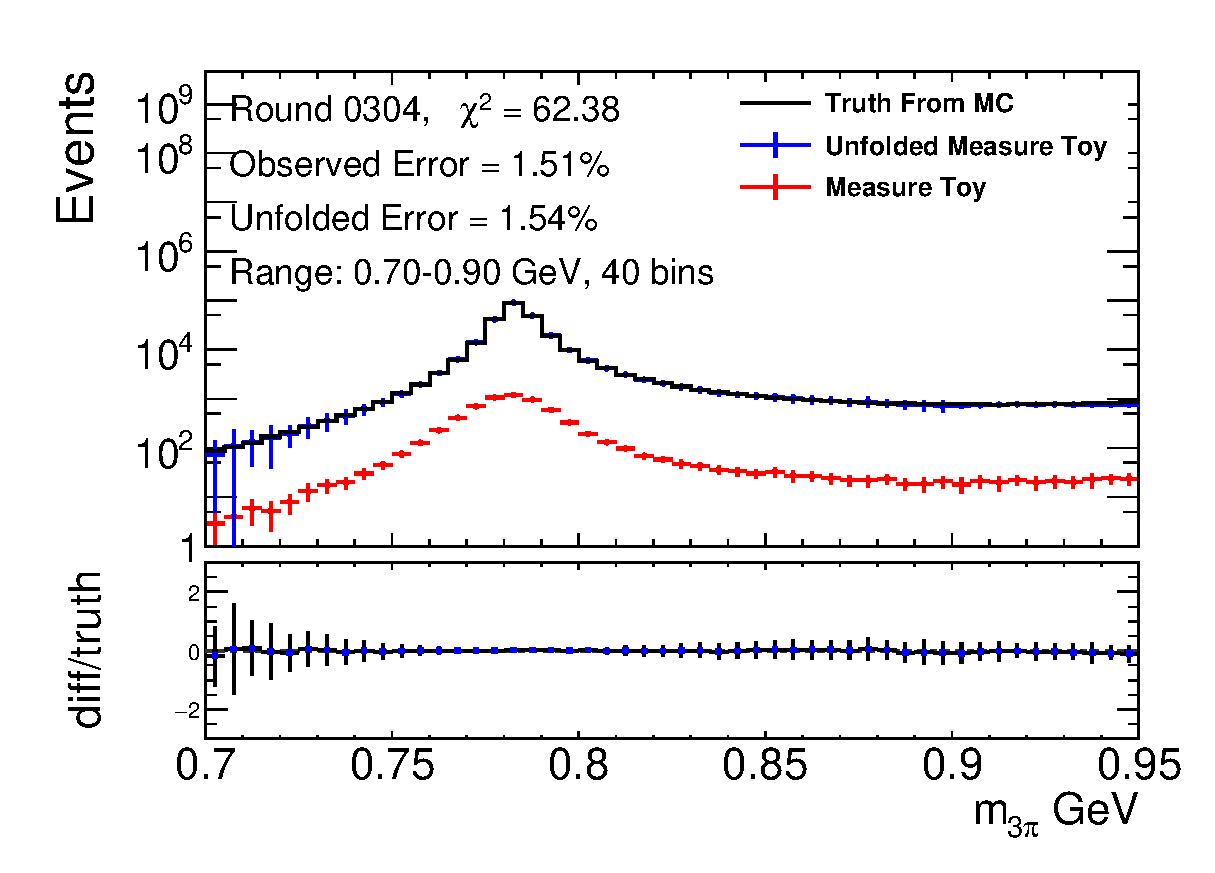
\includegraphics[width=0.32\textwidth]{fig/mc_unfold_round0304_omega.eps}
        \label{fig:unfold_round0304_omega}
    }\hfill
    \subfloat[Round 03/04, $\phi(1020)$ region]{
        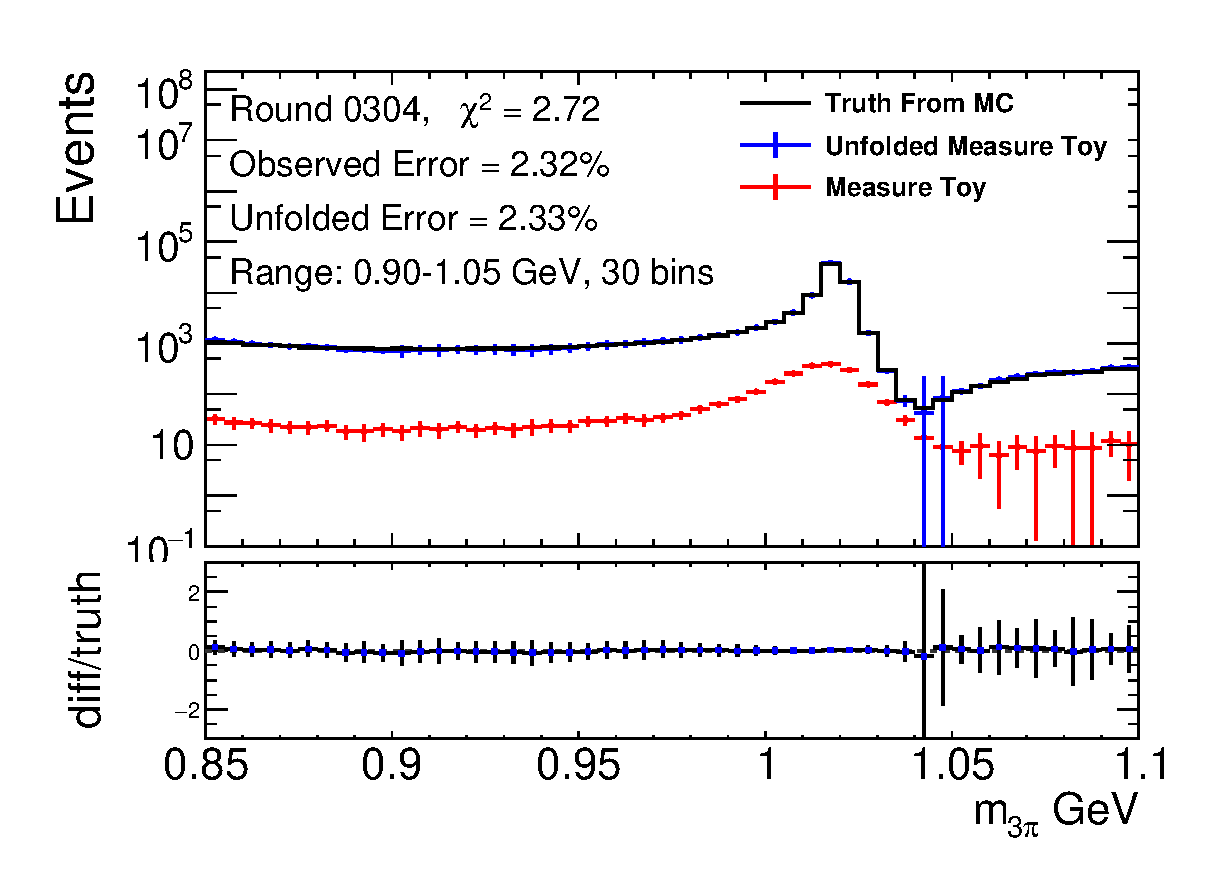
\includegraphics[width=0.32\textwidth]{fig/mc_unfold_round0304_phi.eps}
        \label{fig:unfold_round0304_phi}
    }\hfill
    \subfloat[Round 03/04, $\omega^{\prime}/\omega^{\prime\prime}$ region]{
        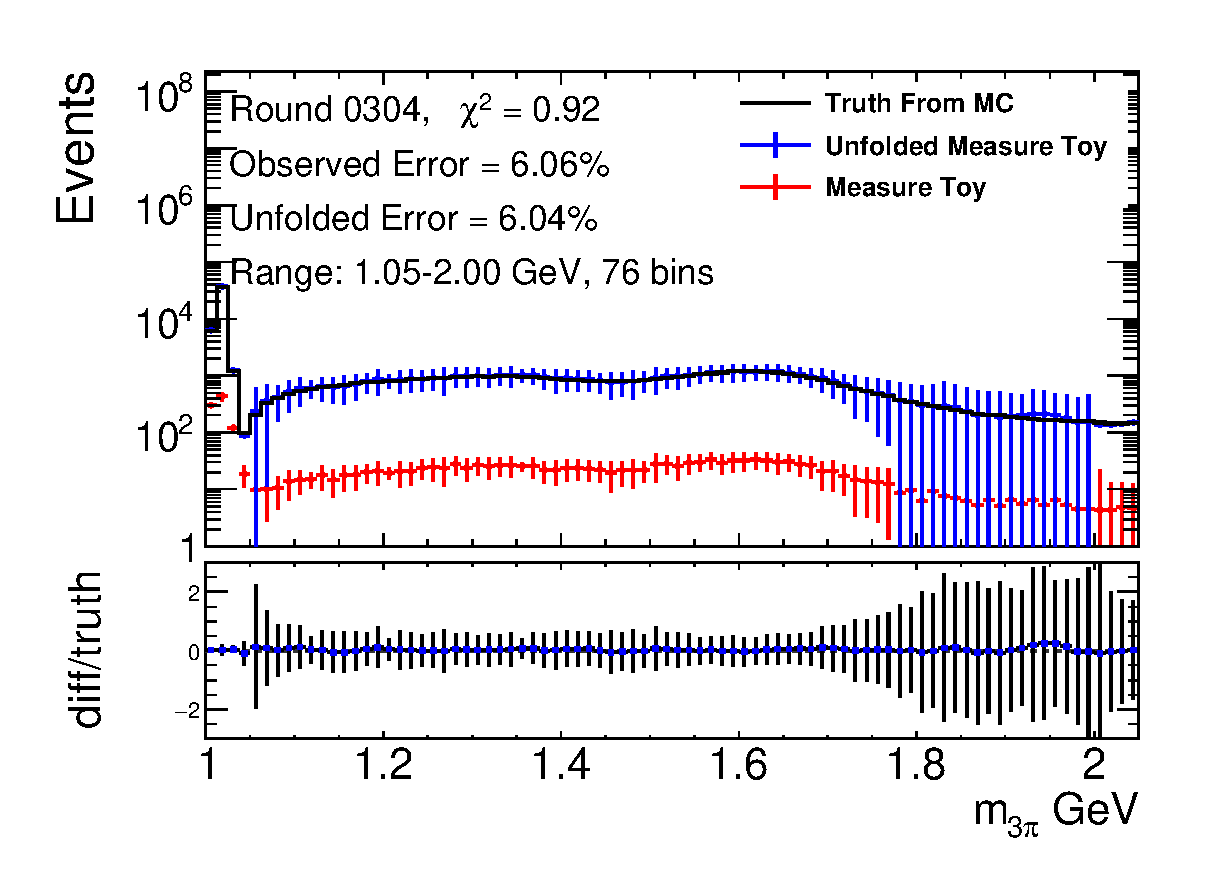
\includegraphics[width=0.32\textwidth]{fig/mc_unfold_round0304_high.eps}
        \label{fig:unfold_round0304_high}
    }

    \vspace{0.5\baselineskip}

    % === Row 2: Round 15 ===
    \subfloat[Round 15, $\omega(782)$ region]{
        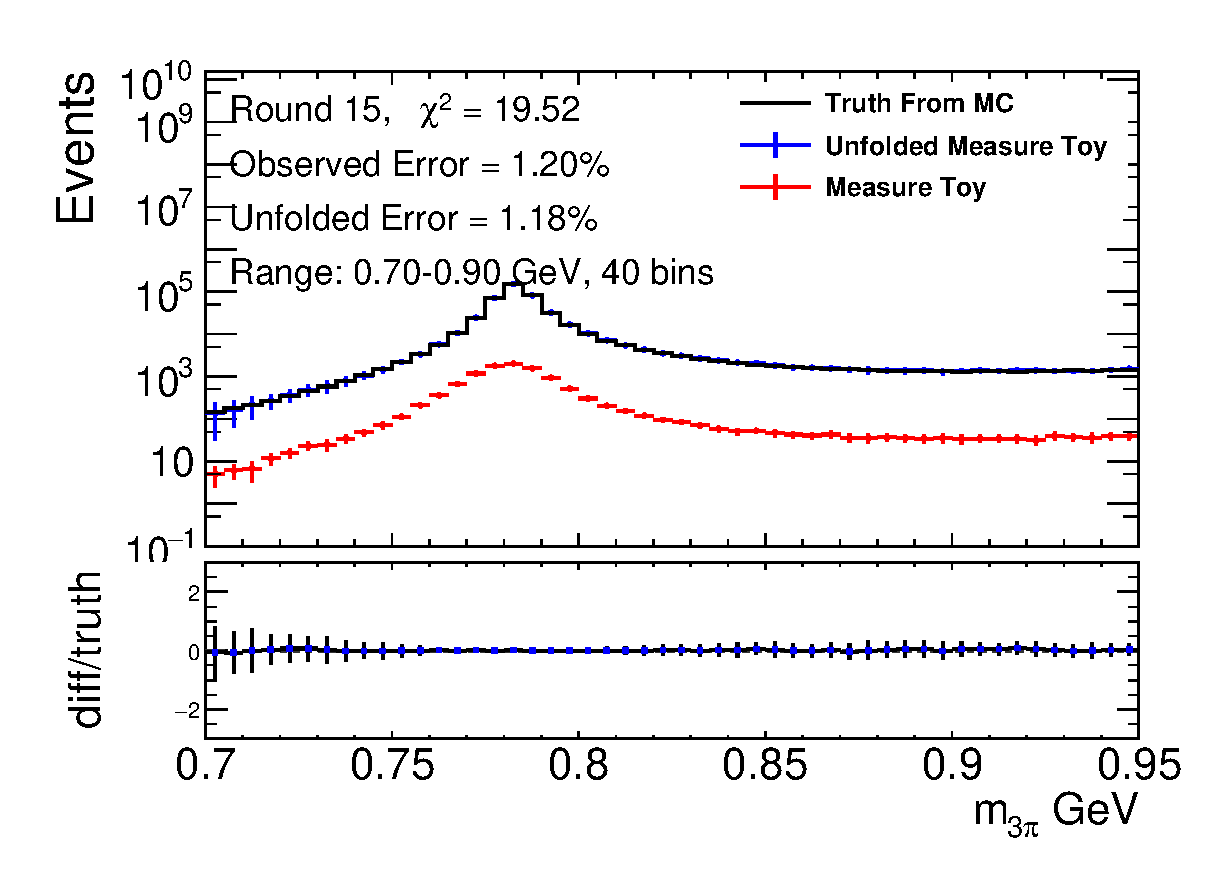
\includegraphics[width=0.32\textwidth]{fig/mc_unfold_round15_omega.eps}
        \label{fig:unfold_round15_omega}
    }\hfill
    \subfloat[Round 15, $\phi(1020)$ region]{
        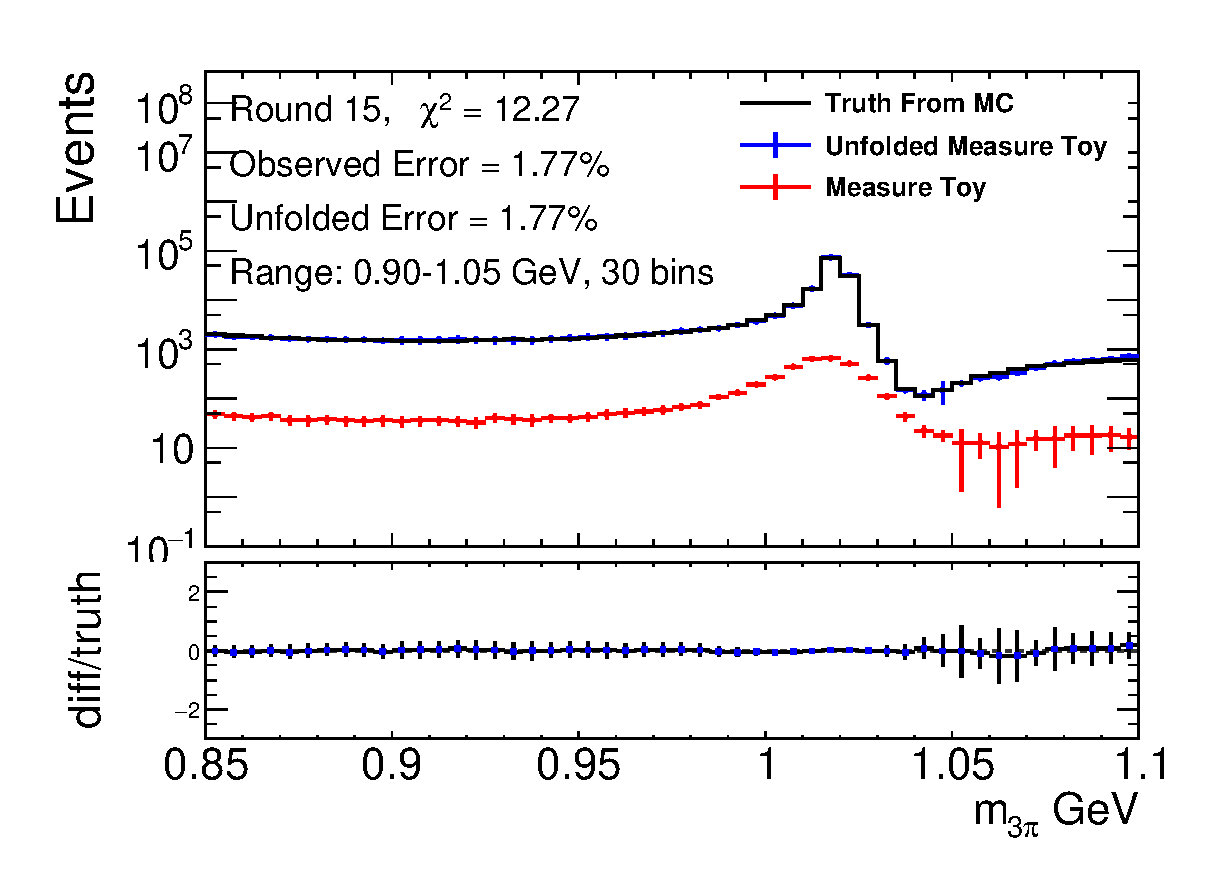
\includegraphics[width=0.32\textwidth]{fig/mc_unfold_round15_phi.eps}
        \label{fig:unfold_round15_phi}
    }\hfill
    \subfloat[Round 15, $\omega^{\prime}/\omega^{\prime\prime}$ region]{
        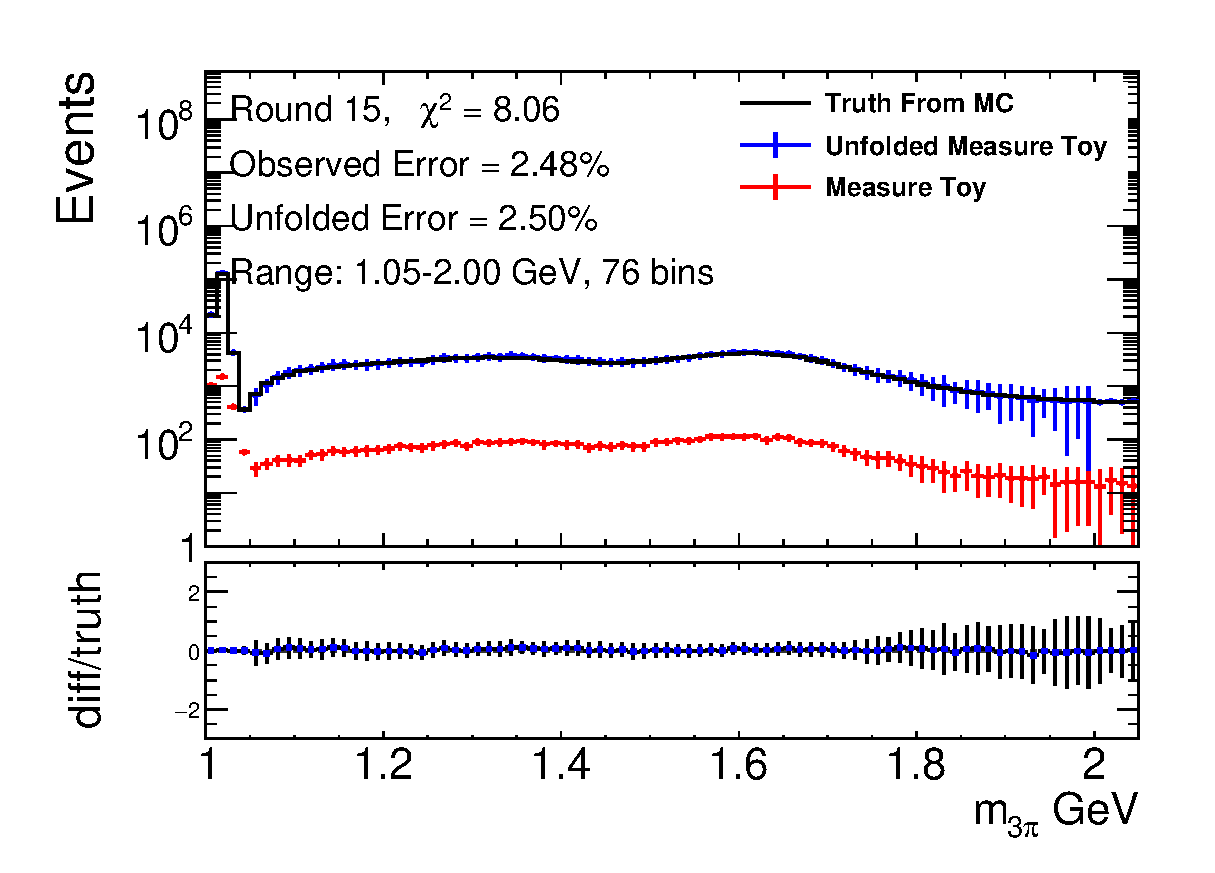
\includegraphics[width=0.32\textwidth]{fig/mc_unfold_round15_high.eps}
        \label{fig:unfold_round15_high}
    }

    \vspace{0.5\baselineskip}

    % === Row 3: Round 16 ===
    \subfloat[Round 16, $\omega(782)$ region]{
        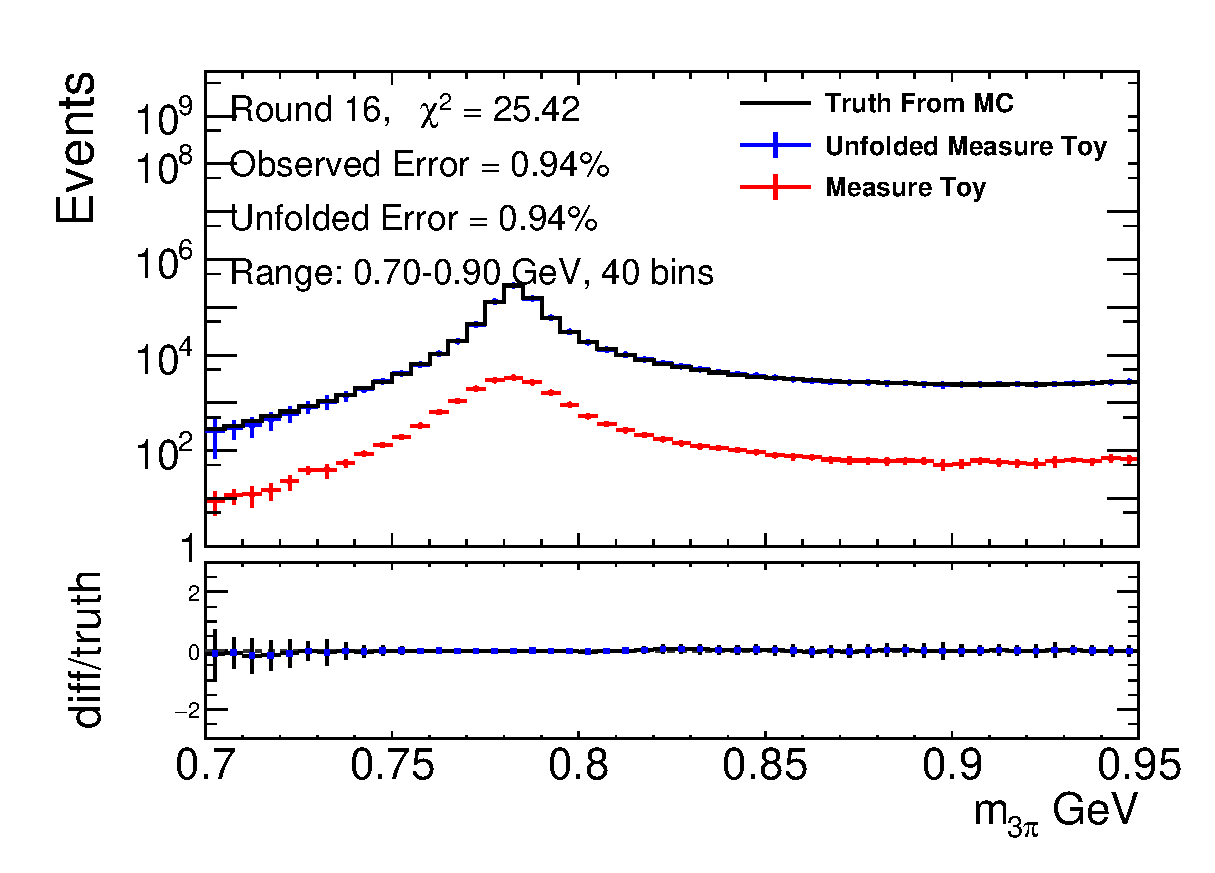
\includegraphics[width=0.32\textwidth]{fig/mc_unfold_round16_omega.eps}
        \label{fig:unfold_round16_omega}
    }\hfill
    \subfloat[Round 16, $\phi(1020)$ region]{
        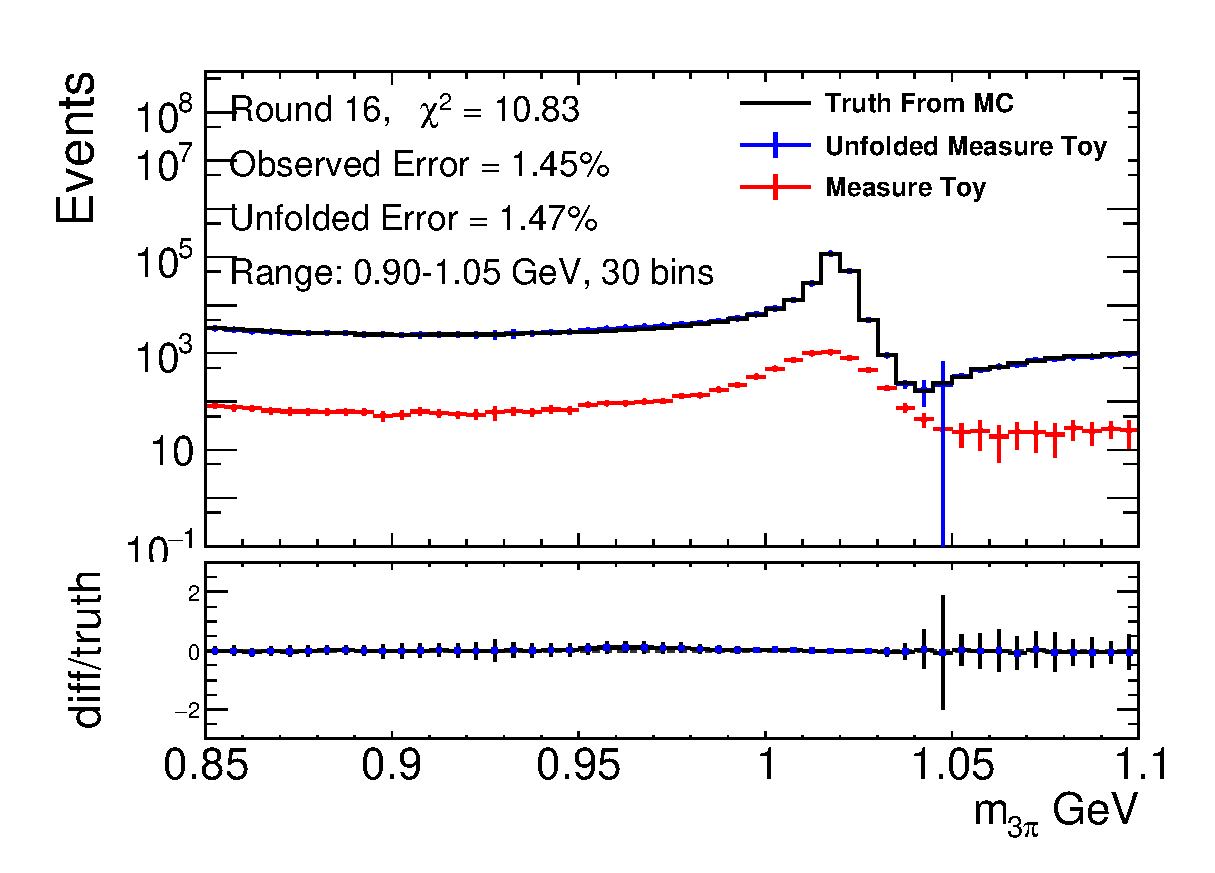
\includegraphics[width=0.32\textwidth]{fig/mc_unfold_round16_phi.eps}
        \label{fig:unfold_round16_phi}
    }\hfill
    \subfloat[Round 16, $\omega^{\prime}/\omega^{\prime\prime}$ region]{
        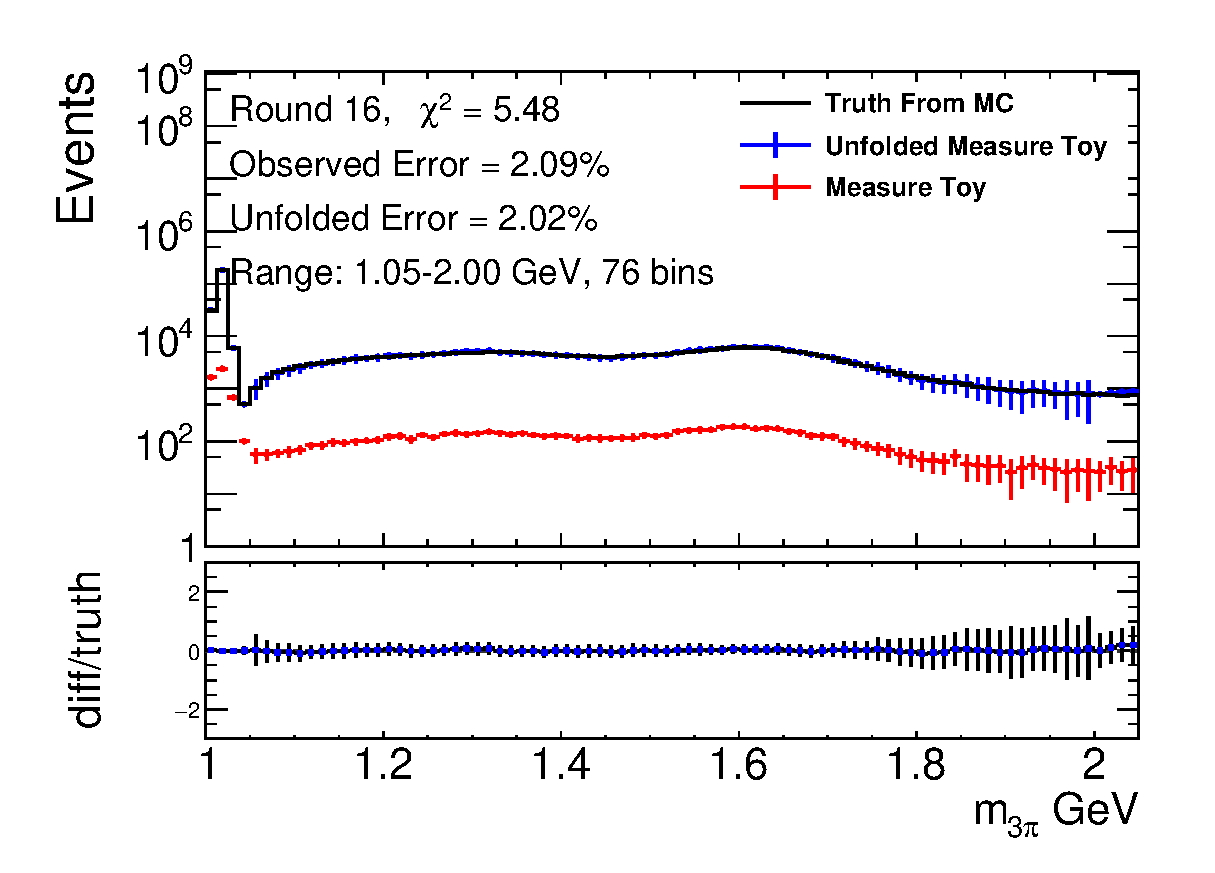
\includegraphics[width=0.32\textwidth]{fig/mc_unfold_round16_high.eps}
        \label{fig:unfold_round16_high}
    }

    \vspace{0.5\baselineskip}

    % === Row 4: Round 17 ===
    \subfloat[Round 17, $\omega(782)$ region]{
        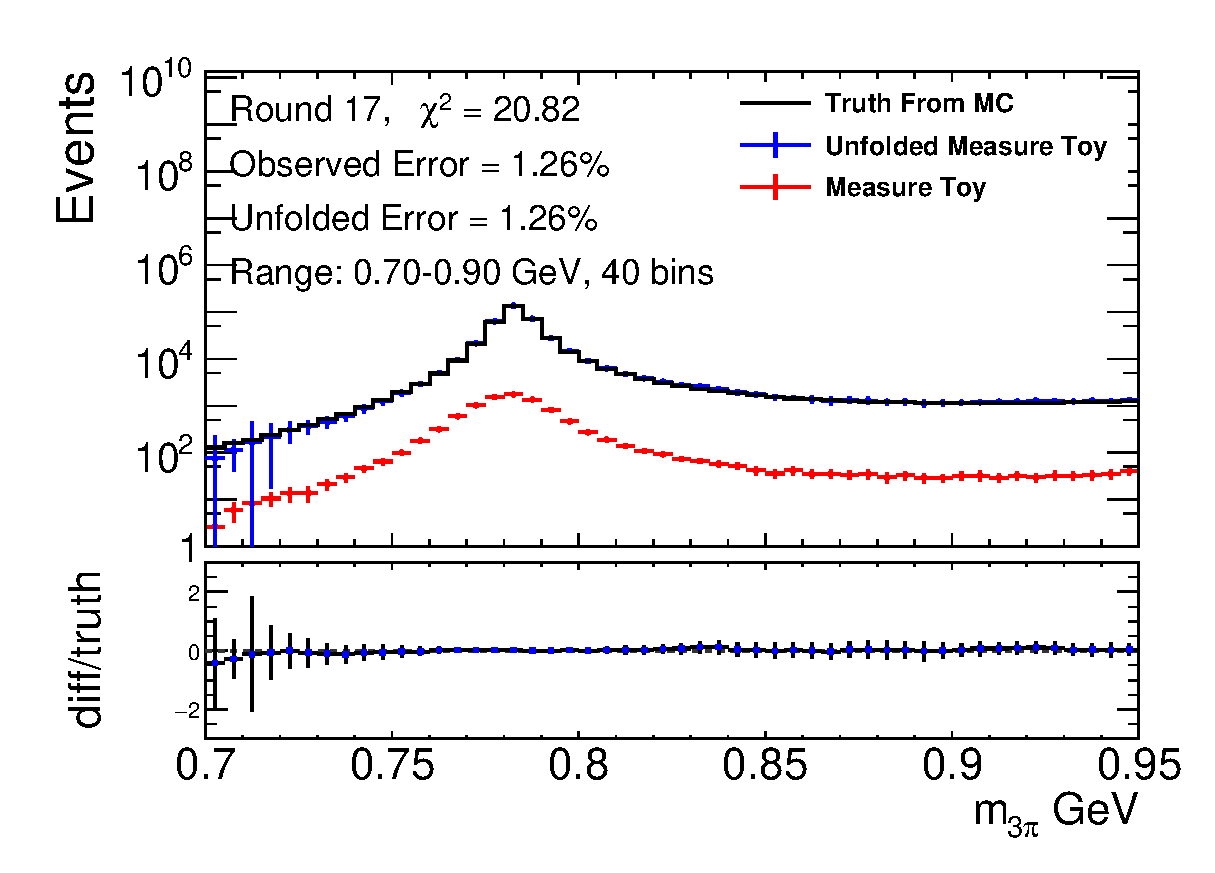
\includegraphics[width=0.32\textwidth]{fig/mc_unfold_round17_omega.eps}
        \label{fig:unfold_round17_omega}
    }\hfill
    \subfloat[Round 17, $\phi(1020)$ region]{
        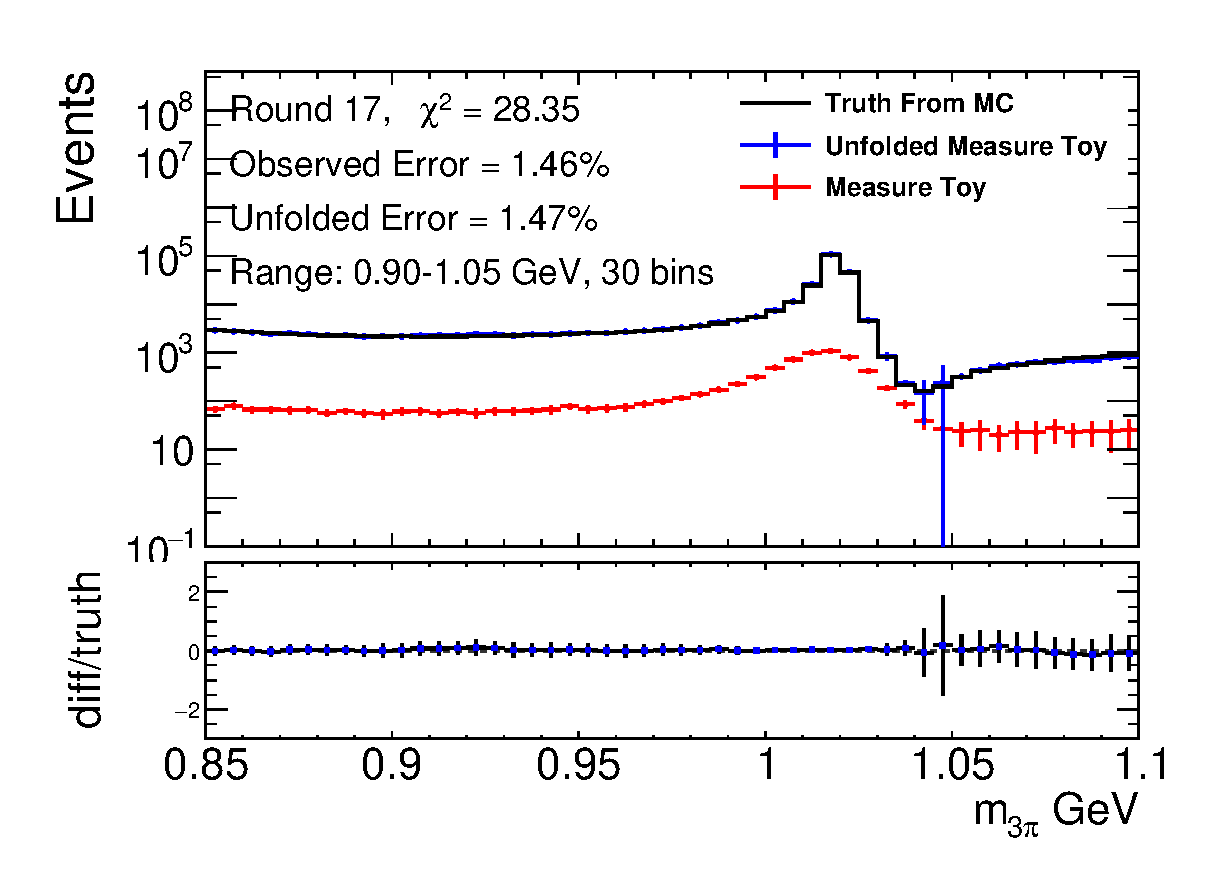
\includegraphics[width=0.32\textwidth]{fig/mc_unfold_round17_phi.eps}
        \label{fig:unfold_round17_phi}
    }\hfill
    \subfloat[Round 17, $\omega^{\prime}/\omega^{\prime\prime}$ region]{
        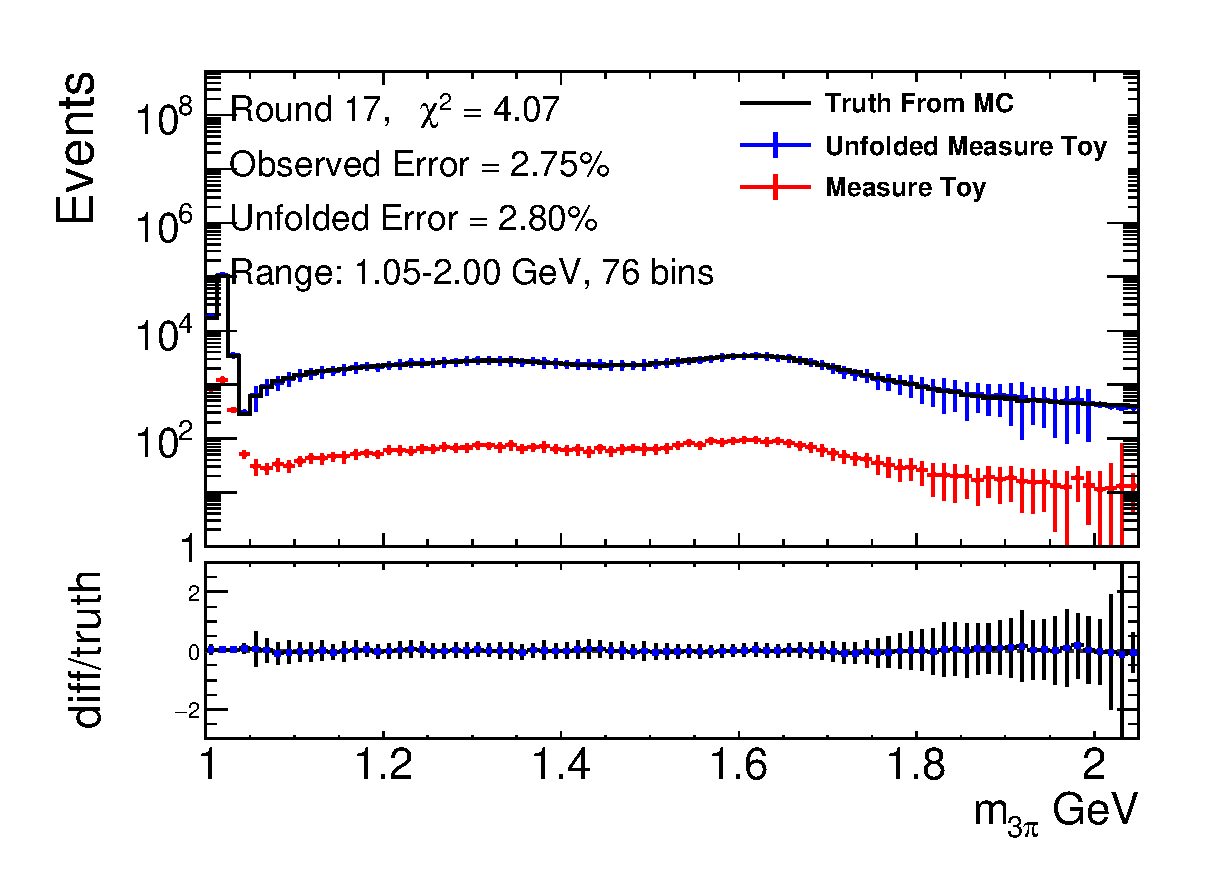
\includegraphics[width=0.32\textwidth]{fig/mc_unfold_round17_high.eps}
        \label{fig:unfold_round17_high}
    }

    \caption{Unfolded results for four data-taking periods (Round~03/04, Round~15, Round~16, Round~17) using the IDS method. The unfolding parameters were optimized using the Round~16 MC sample (third row) and then applied to all rounds.}
    \label{fig:mc_unfold_results_all_rounds}
\end{figure}

To further validate the unfolding procedure, we compare the relative
statistical uncertainty of the unfolded spectrum with that of the test MC
sample. The relative uncertainty of the test MC spectrum,
$\delta_{\text{test}}$, is computed by summing in quadrature the Poisson errors
of each bin and dividing by the total yield:
\begin{equation}
    \delta_{\text{test}} = \frac{\sqrt{\sum_{i} \sigma_i^2}}{\sum_i N_i},
\end{equation}
where $N_i$ and $\sigma_i$ are the content and Poisson error of bin $i$ in the test MC distribution, respectively. This represents the Poisson statistical uncertainty of the test MC sample.

The relative uncertainty of the unfolded spectrum, $\delta_{\text{unfolded}}$,
is derived from the full covariance matrix $\Sigma$ obtained from the toy MC
ensemble:
\begin{equation}
    \delta_{\text{unfolded}} = \frac{\sqrt{\sum_{i,j} \Sigma_{ij}}}{\sum_i u_i},
\end{equation}
where $u_i$ are the bin contents of the unfolded spectrum. The relative uncertainty of the unfolded spectrum should not be smaller than the Poisson uncertainty of the test MC sample.

% The extracted signal yields after applying the $\chi^2_{4C}$ correction and selection are shown in Fig.~\ref{fig:signal_yields_corr} as a function of $M_{3\pi}$. It should be noted that the helix parameter corrections are applied only to the signal MC samples, while the data events remain uncorrected. Clear peaks corresponding to the $\omega(782)$ and $\phi(1020)$ resonances are observed, while the higher-mass region exhibits broader structures indicative of excited $\omega$ states.

% \begin{figure}[htbp]
% \centering
% \subfloat[$\omega(782)$ region]{
% 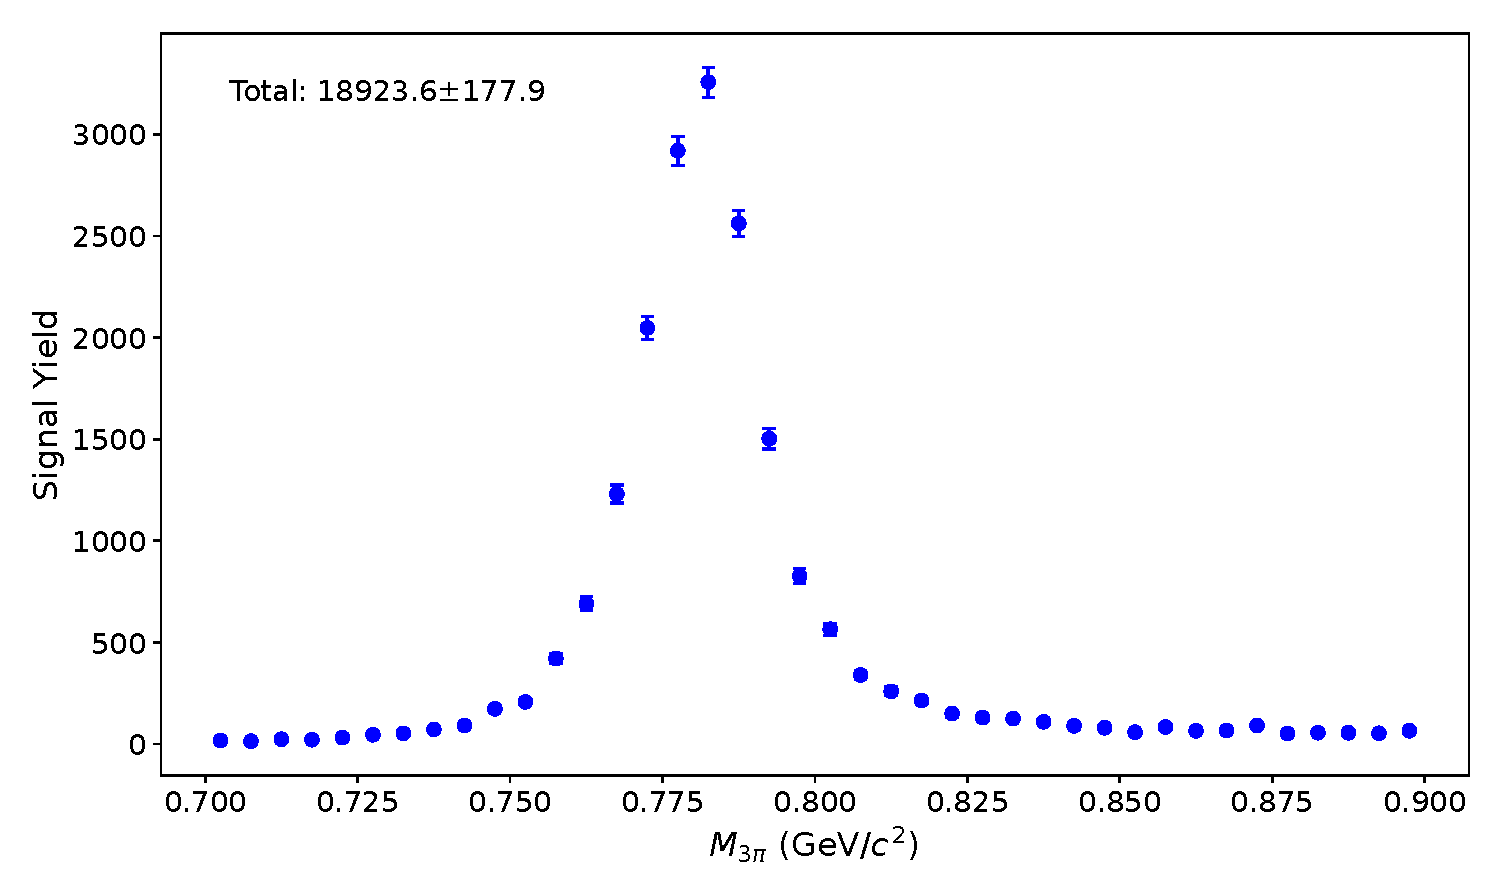
\includegraphics[width=0.32\textwidth]{fig/yields_omega_corr.eps}
% \label{fig:yields_omega_corr}
% }
% \hfill
% \subfloat[$\phi(1020)$ region]{
% 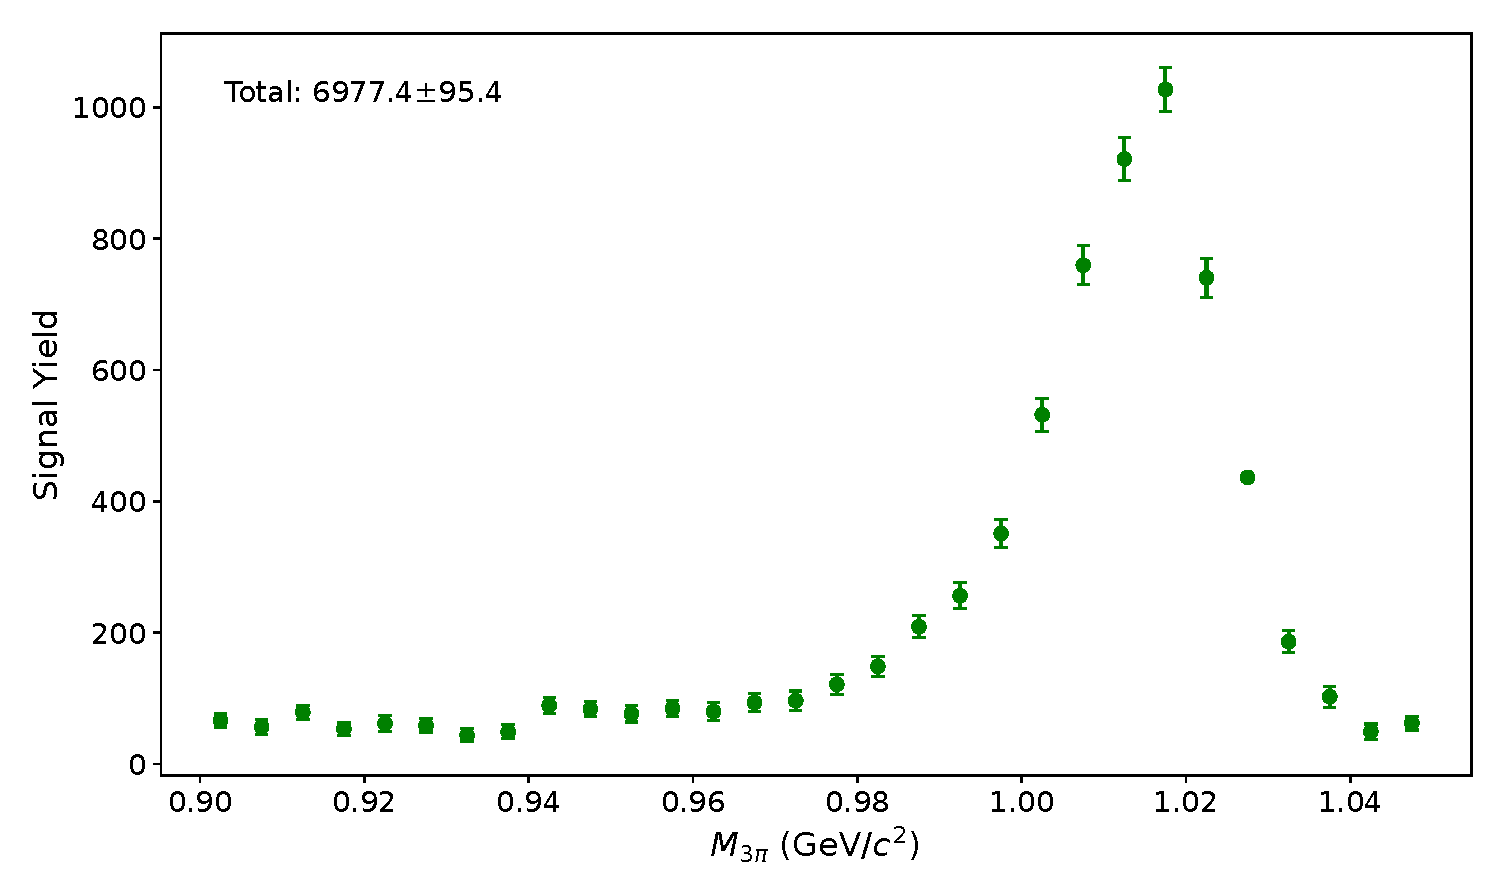
\includegraphics[width=0.32\textwidth]{fig/yields_phi_corr.eps}
% \label{fig:yields_phi_corr}
% }
% \hfill
% \subfloat[$\omega^{\prime}/\omega^{\prime\prime}$ region]{
% 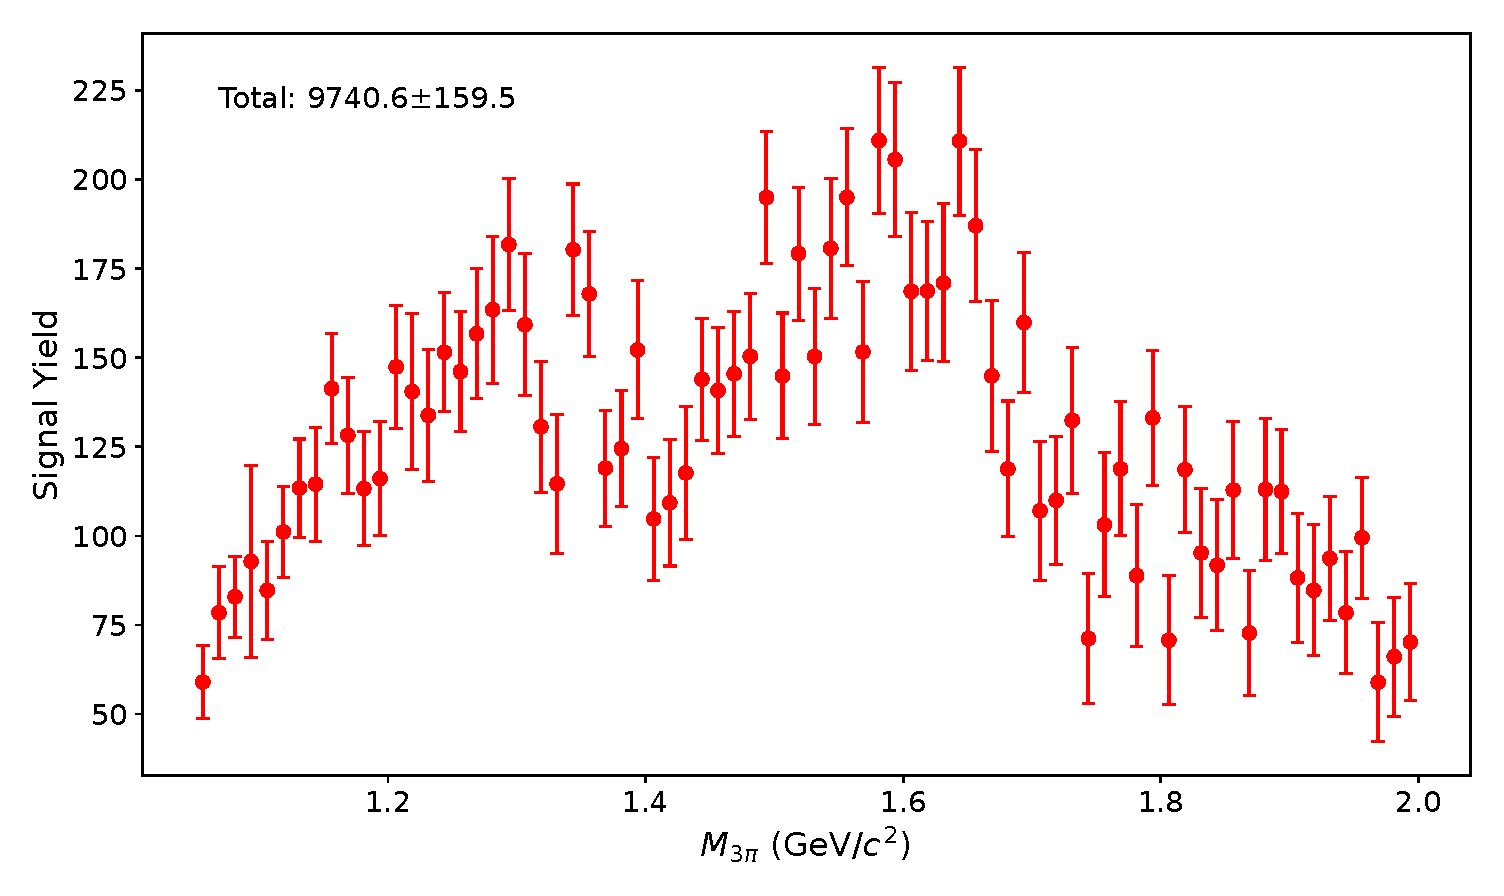
\includegraphics[width=0.32\textwidth]{fig/yields_high_corr.eps}
% \label{fig:yields_high_corr}
% }
% \caption{Extracted signal yields as a function of $M_{3\pi}$ after applying helix parameter corrections to the signal MC and the $\chi^2_{4C} < 50$ selection requirement. The three mass regions are shown separately. The error bars represent the statistical uncertainties from the fits. The $\omega(782)$ and $\phi(1020)$ resonances appear as clear peaks, while the higher-mass region reveals broader structures corresponding to excited $\omega$ states.}
% \label{fig:signal_yields_corr}
% \end{figure}


Using the corrected migration matrix $A_{ij}^{\text{corr}}$, the unfolding of the $M_{3\pi}$ distribution is performed on data from Sec.~\ref{DataYields}. The unfolding procedure automatically accounts for the reconstruction and selection efficiency of the signal by incorporating information from missing events, rather than relying on the response matrix alone. The mass range for each resonance region is extended during the unfolding procedure and subsequently truncated back to the nominal interval defined in Tab.~\ref{tab:optimized_parameters} for the final results. Figure~\ref{fig:unfolded_data_results_all_rounds} presents the unfolded $M_{3\pi}$ distributions for data in the three regions.

% 添加结果图（四个数据周期，三个物理区域）
\begin{figure}[htbp]
\centering

% === Row 1: Round 03/04 ===
\subfloat[Round 03/04, $\omega(782)$ region]{
    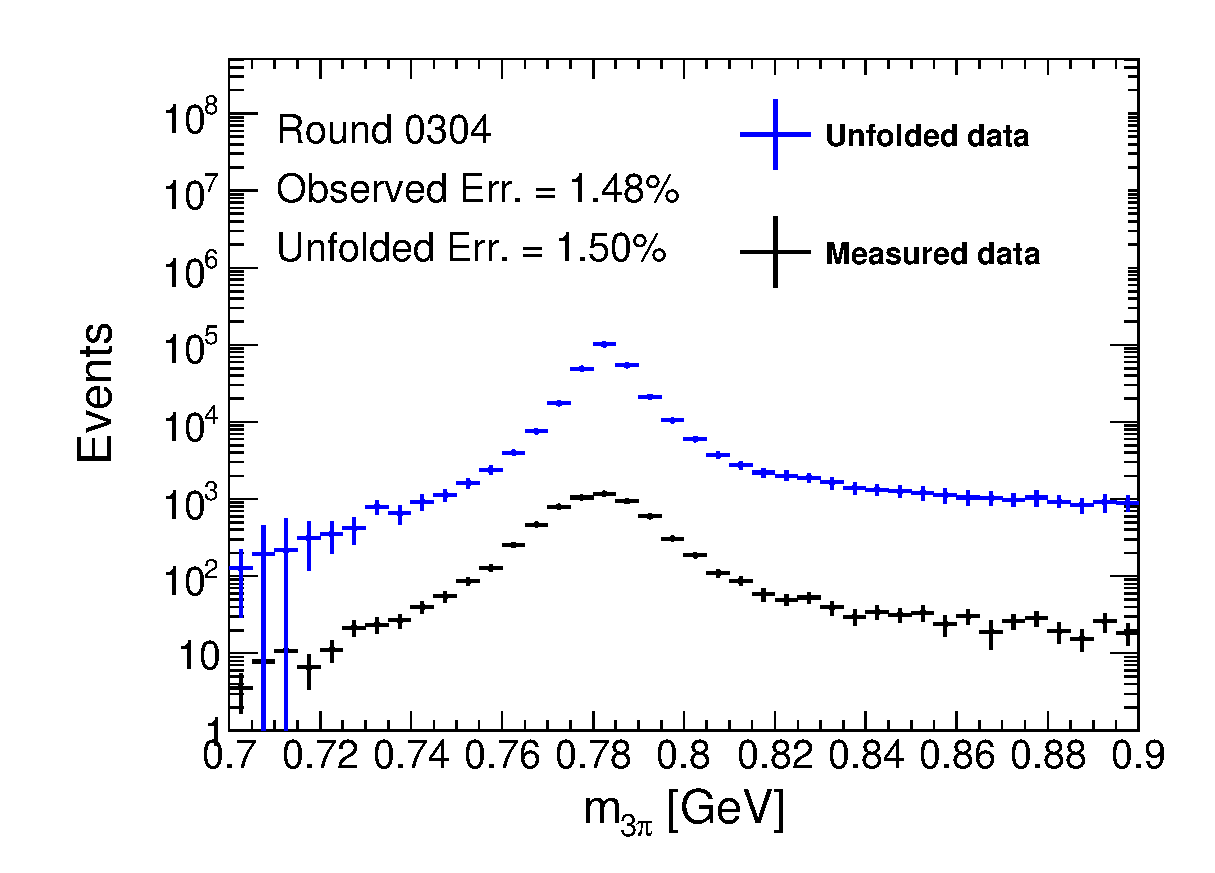
\includegraphics[width=0.32\textwidth]{fig/unfolded_omega_round0304.eps}
    \label{fig:unfolded_omega_r0304}
}\hfill
\subfloat[Round 03/04, $\phi(1020)$ region]{
    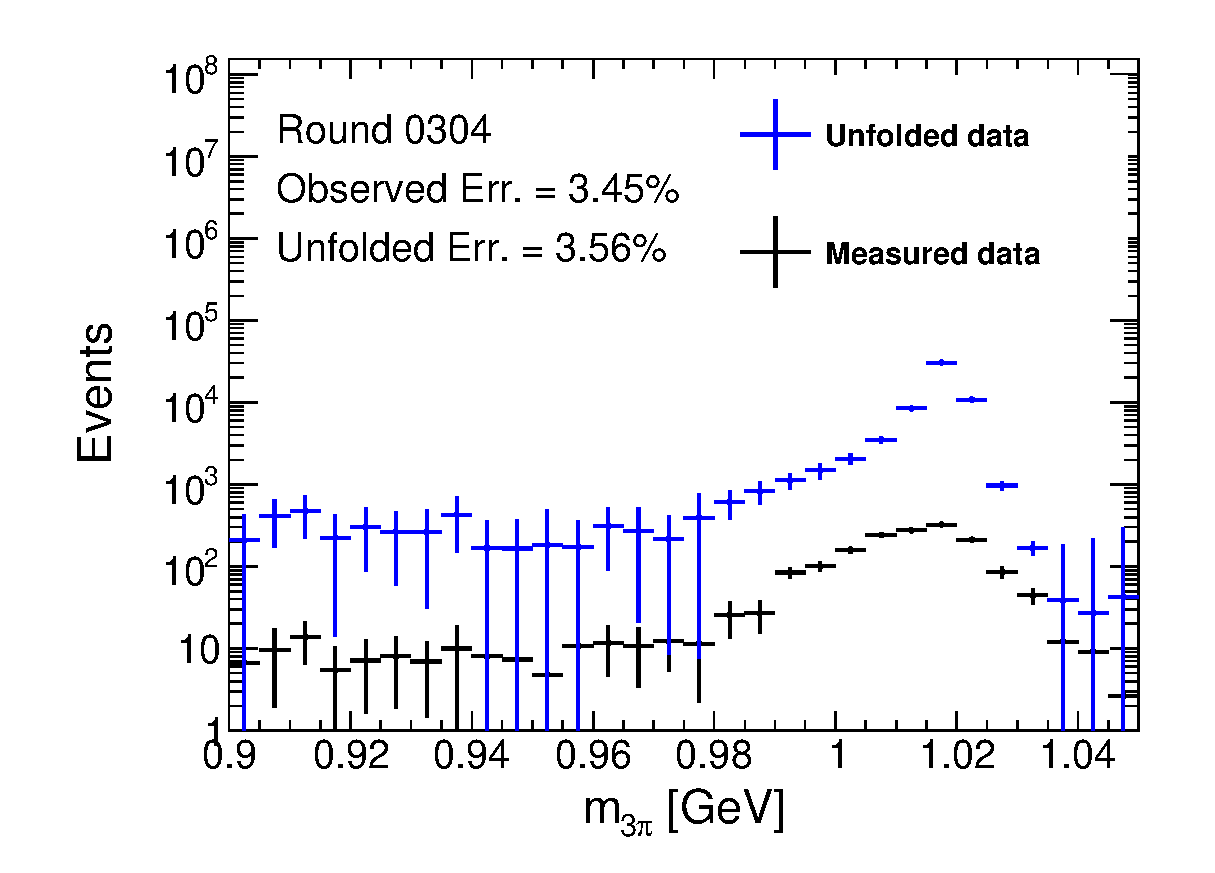
\includegraphics[width=0.32\textwidth]{fig/unfolded_phi_round0304.eps}
    \label{fig:unfolded_phi_r0304}
}\hfill
\subfloat[Round 03/04, $\omega^{\prime}/\omega^{\prime\prime}$ region]{
    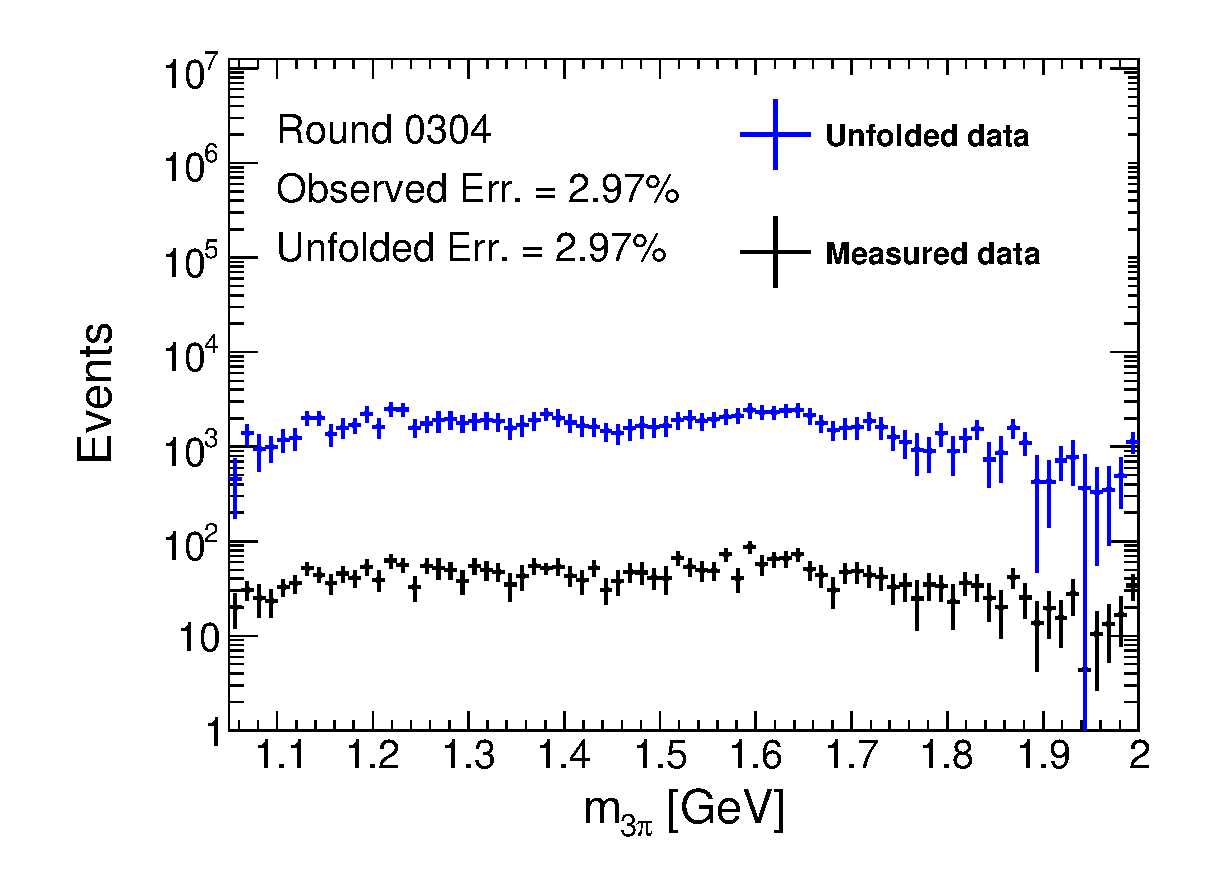
\includegraphics[width=0.32\textwidth]{fig/unfolded_high_round0304.eps}
    \label{fig:unfolded_high_r0304}
}

\vspace{0.5\baselineskip}

% === Row 2: Round 15 ===
\subfloat[Round 15, $\omega(782)$ region]{
    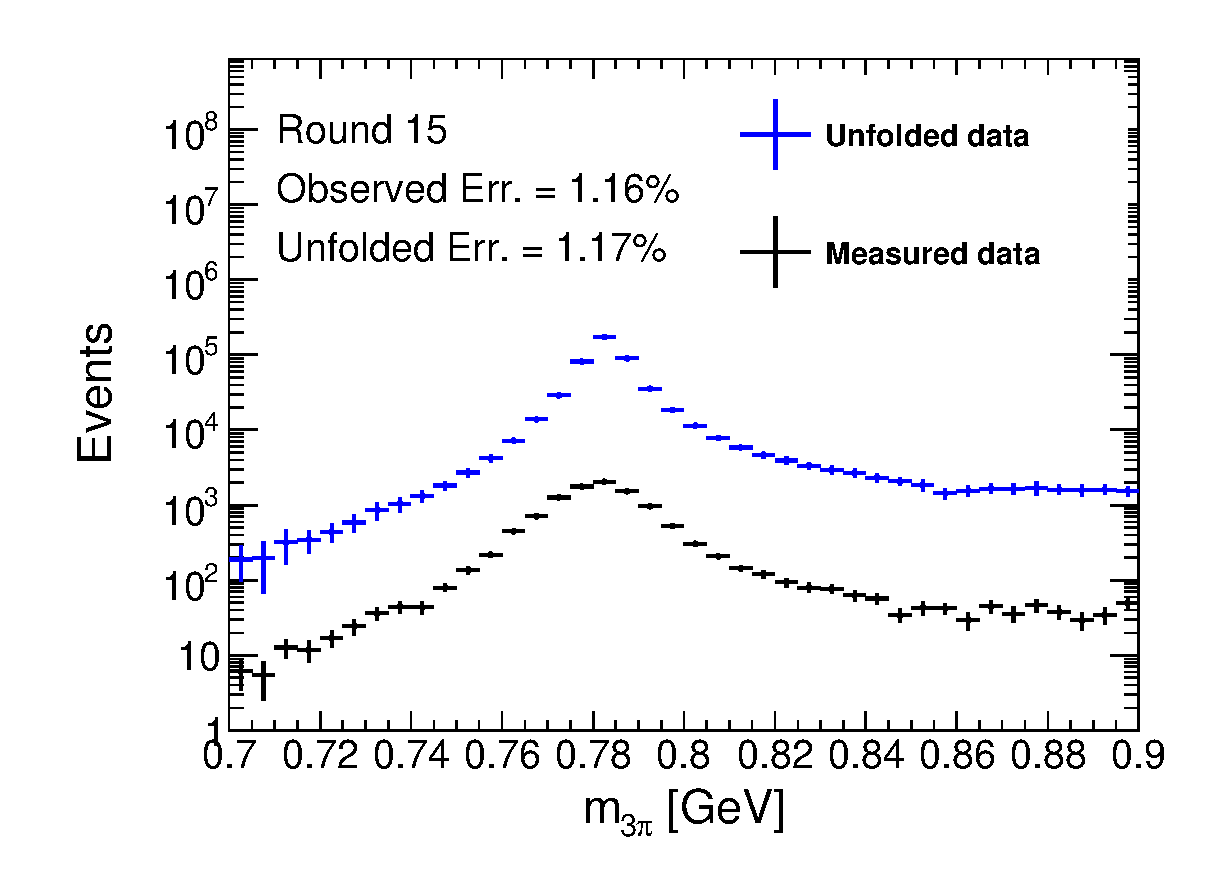
\includegraphics[width=0.32\textwidth]{fig/unfolded_omega_round15.eps}
    \label{fig:unfolded_omega_r15}
}\hfill
\subfloat[Round 15, $\phi(1020)$ region]{
    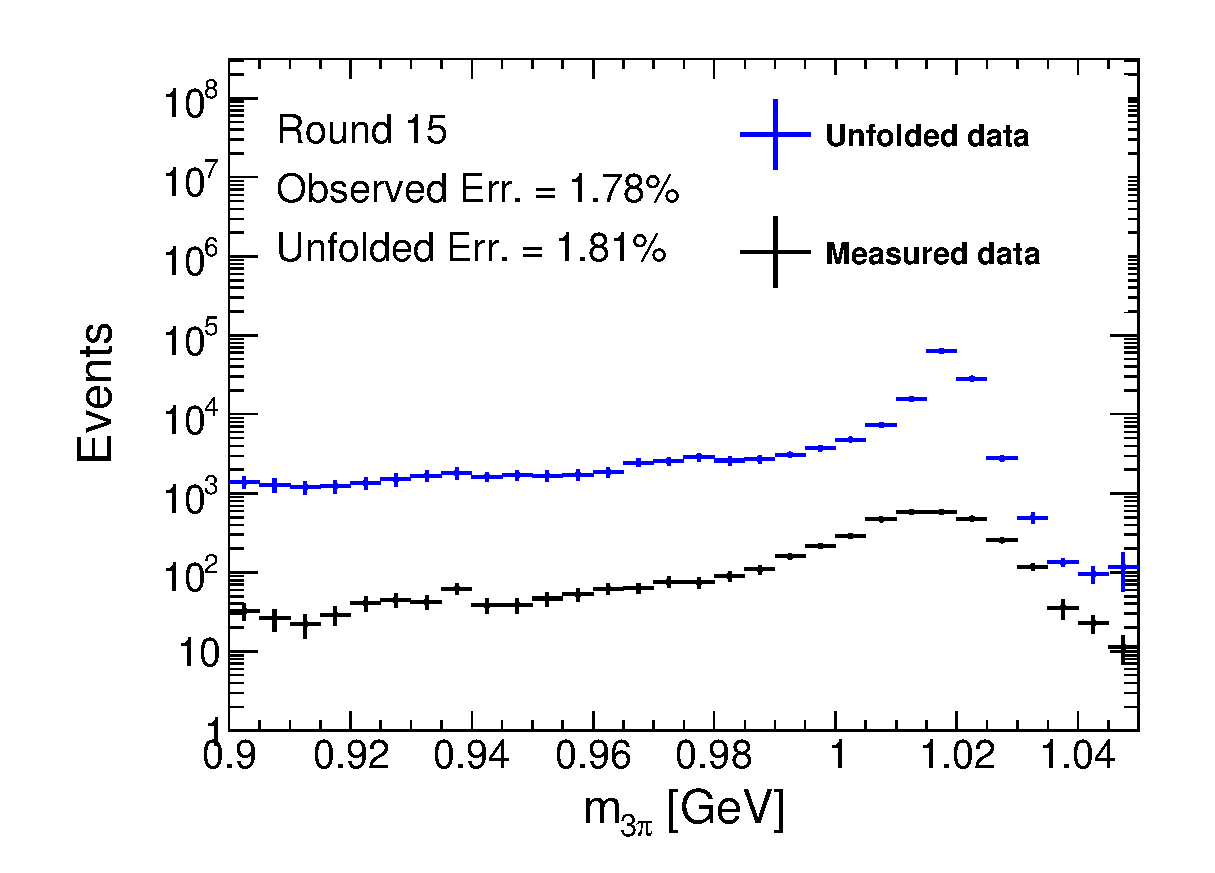
\includegraphics[width=0.32\textwidth]{fig/unfolded_phi_round15.eps}
    \label{fig:unfolded_phi_r15}
}\hfill
\subfloat[Round 15, $\omega^{\prime}/\omega^{\prime\prime}$ region]{
    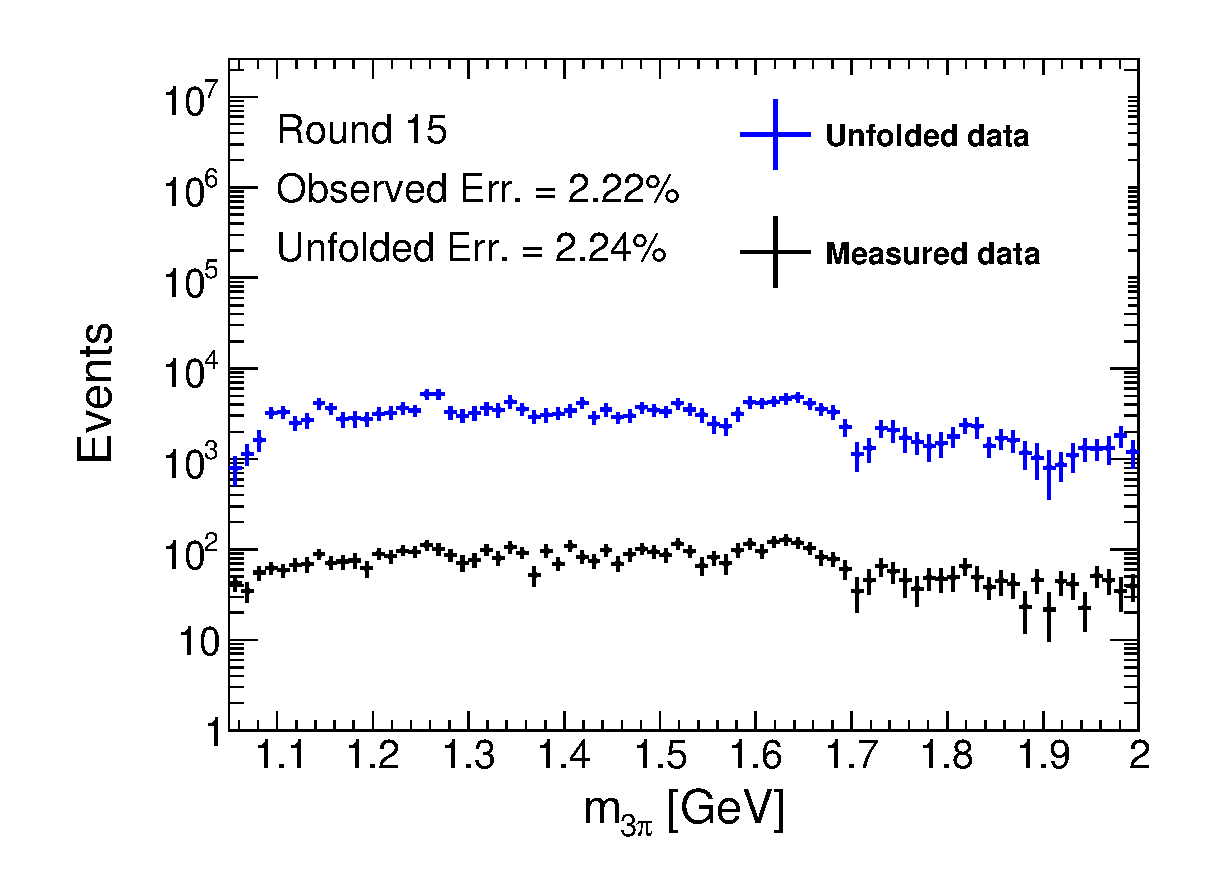
\includegraphics[width=0.32\textwidth]{fig/unfolded_high_round15.eps}
    \label{fig:unfolded_high_r15}
}

\vspace{0.5\baselineskip}

% === Row 3: Round 16 ===
\subfloat[Round 16, $\omega(782)$ region]{
    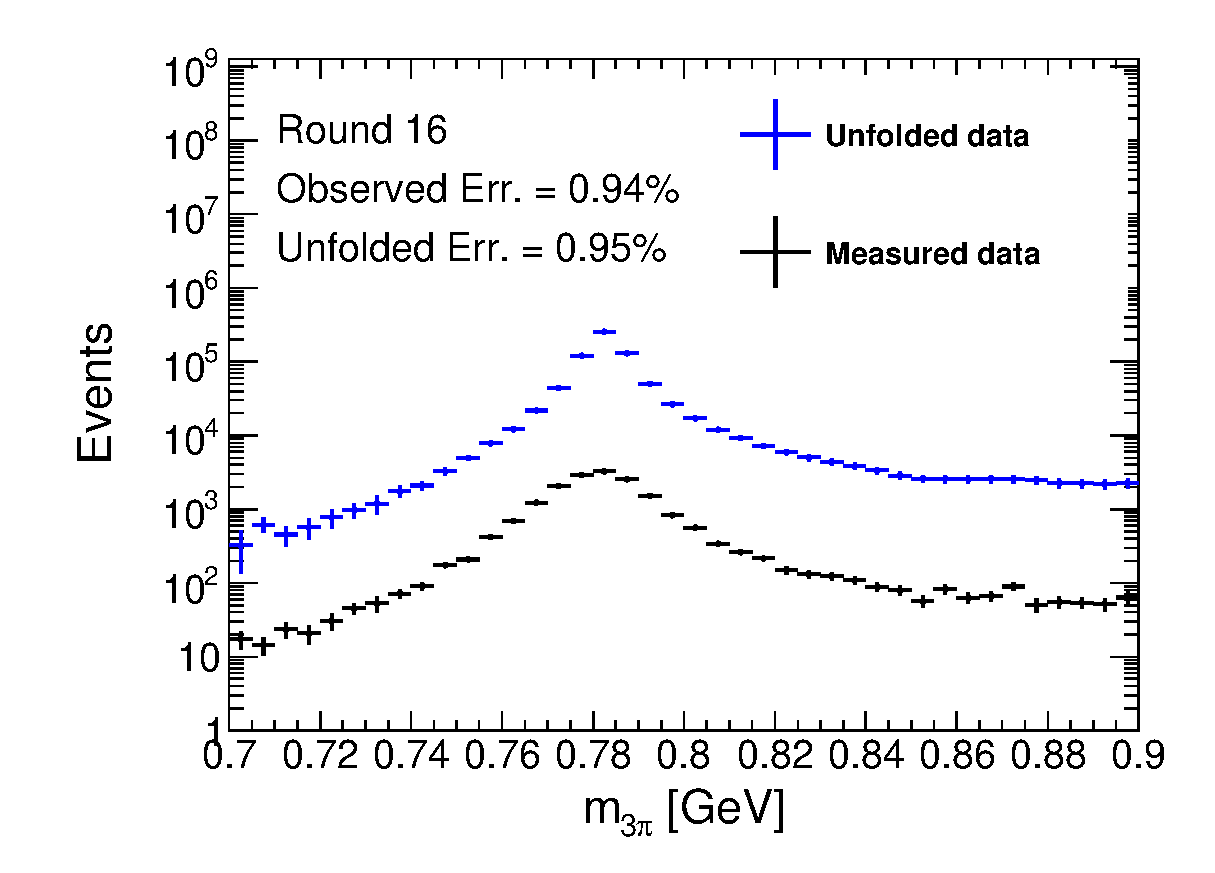
\includegraphics[width=0.32\textwidth]{fig/unfolded_omega_round16.eps}
    \label{fig:unfolded_omega_r16}
}\hfill
\subfloat[Round 16, $\phi(1020)$ region]{
    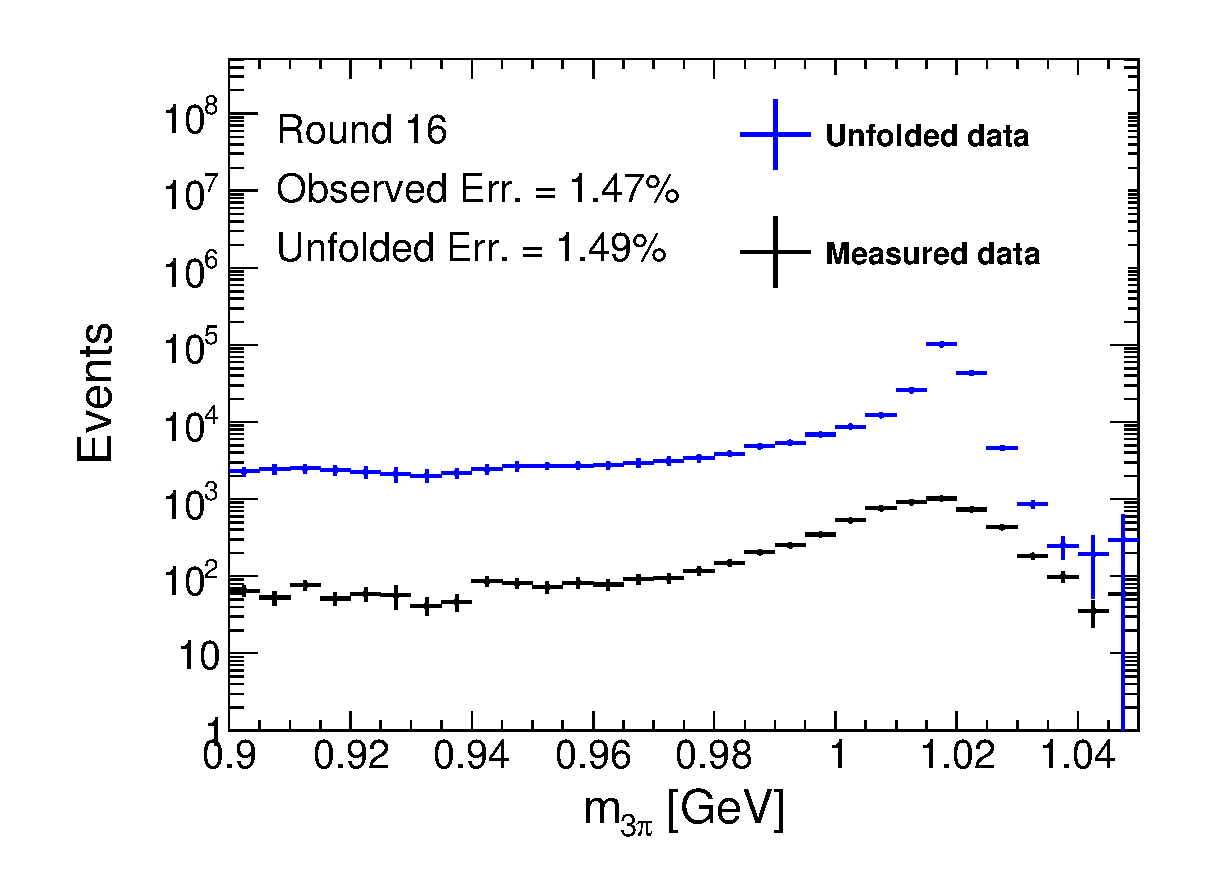
\includegraphics[width=0.32\textwidth]{fig/unfolded_phi_round16.eps}
    \label{fig:unfolded_phi_r16}
}\hfill
\subfloat[Round 16, $\omega^{\prime}/\omega^{\prime\prime}$ region]{
    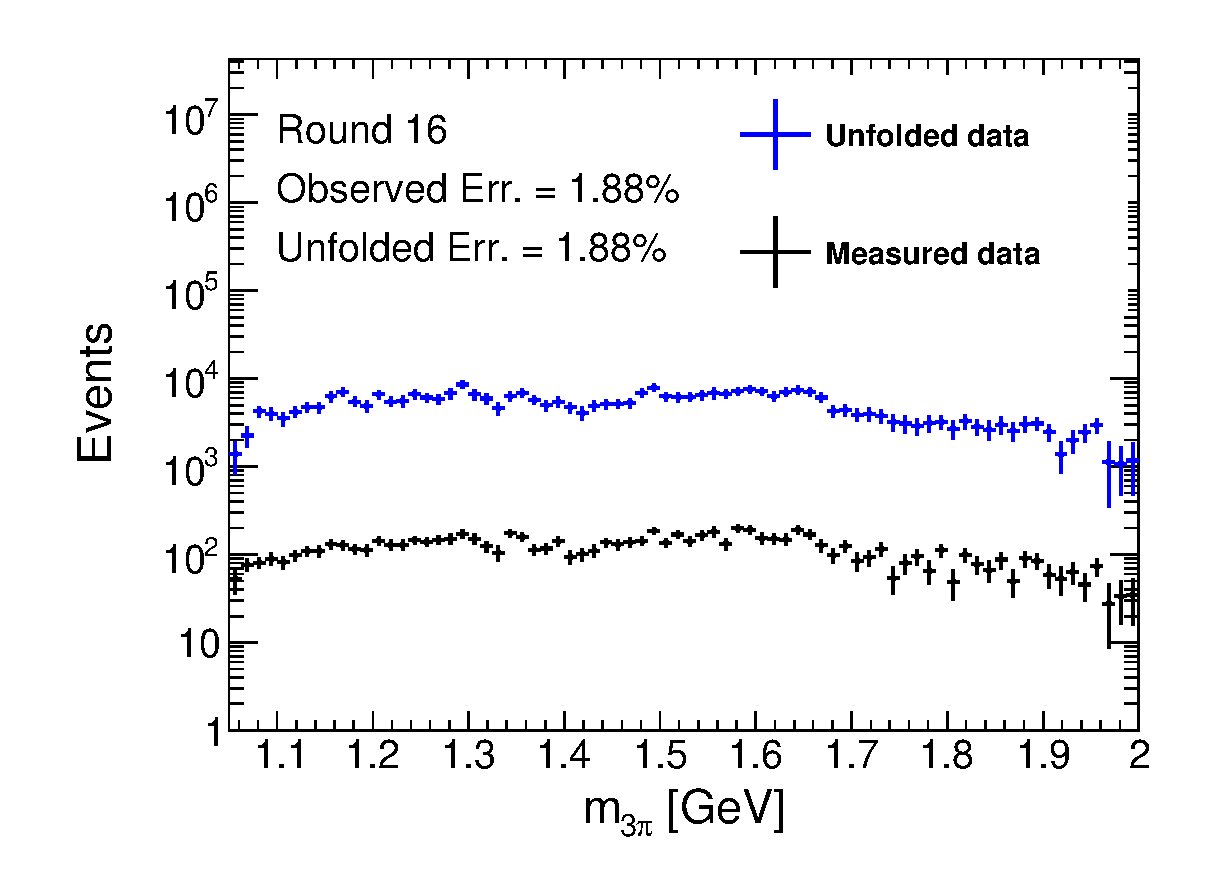
\includegraphics[width=0.32\textwidth]{fig/unfolded_high_round16.eps}
    \label{fig:unfolded_high_r16}
}

\vspace{0.5\baselineskip}

% === Row 4: Round 17 ===
\subfloat[Round 17, $\omega(782)$ region]{
    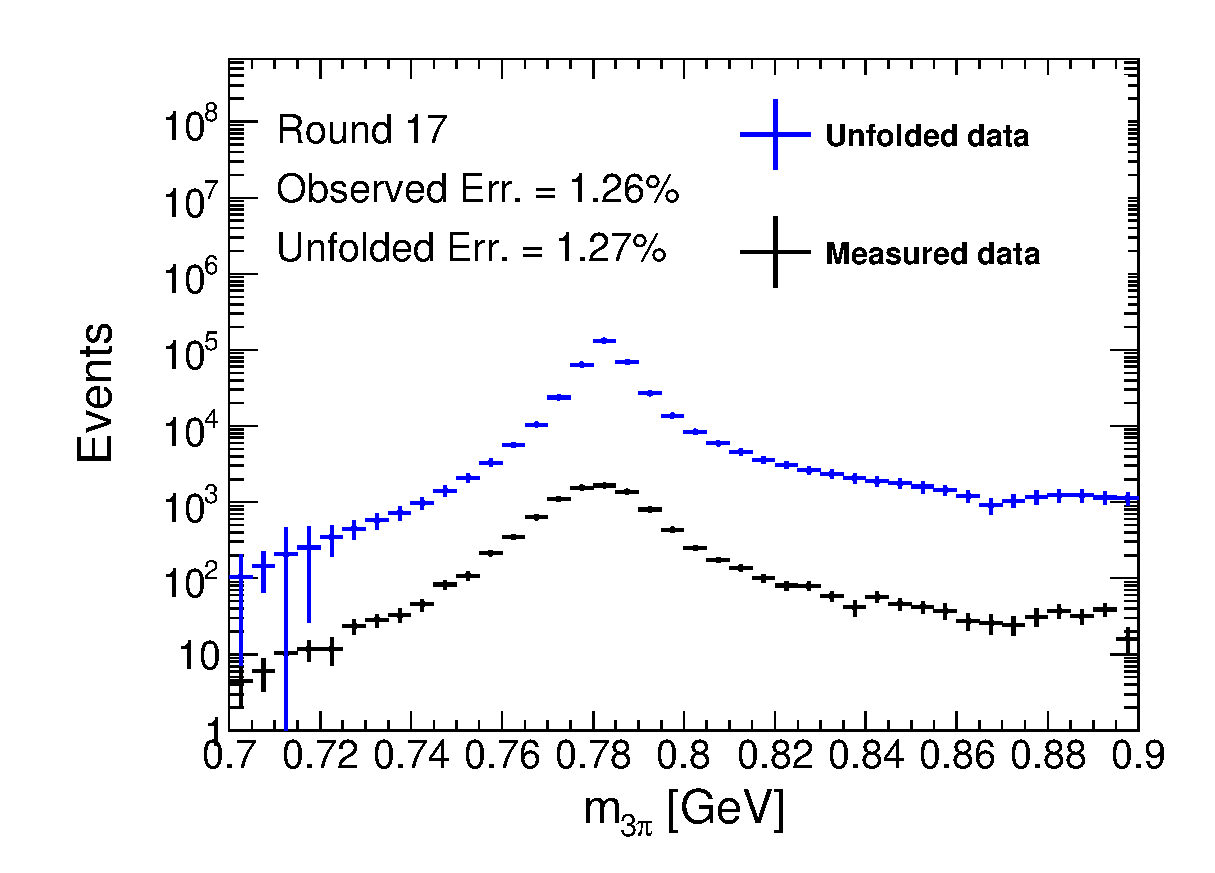
\includegraphics[width=0.32\textwidth]{fig/unfolded_omega_round17.eps}
    \label{fig:unfolded_omega_r17}
}\hfill
\subfloat[Round 17, $\phi(1020)$ region]{
    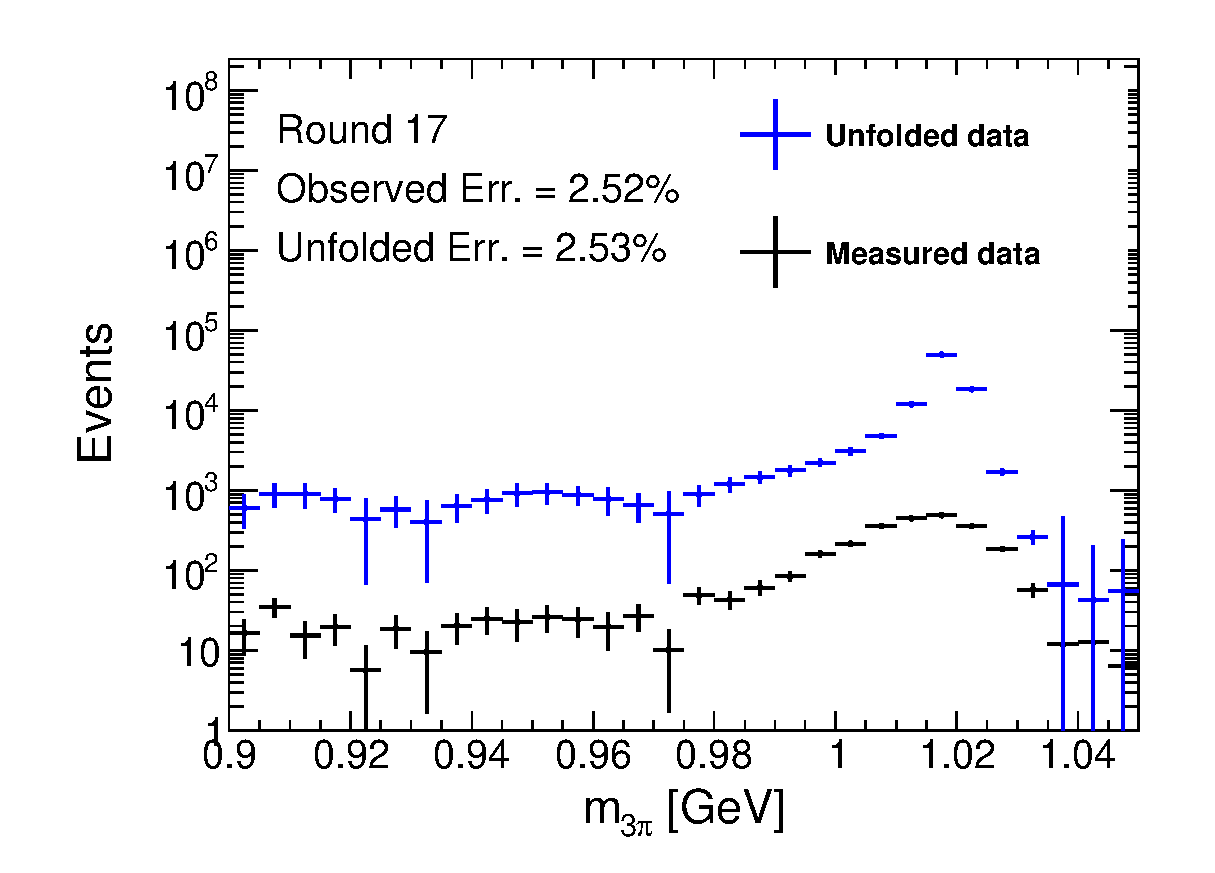
\includegraphics[width=0.32\textwidth]{fig/unfolded_phi_round17.eps}
    \label{fig:unfolded_phi_r17}
}\hfill
\subfloat[Round 17, $\omega^{\prime}/\omega^{\prime\prime}$ region]{
    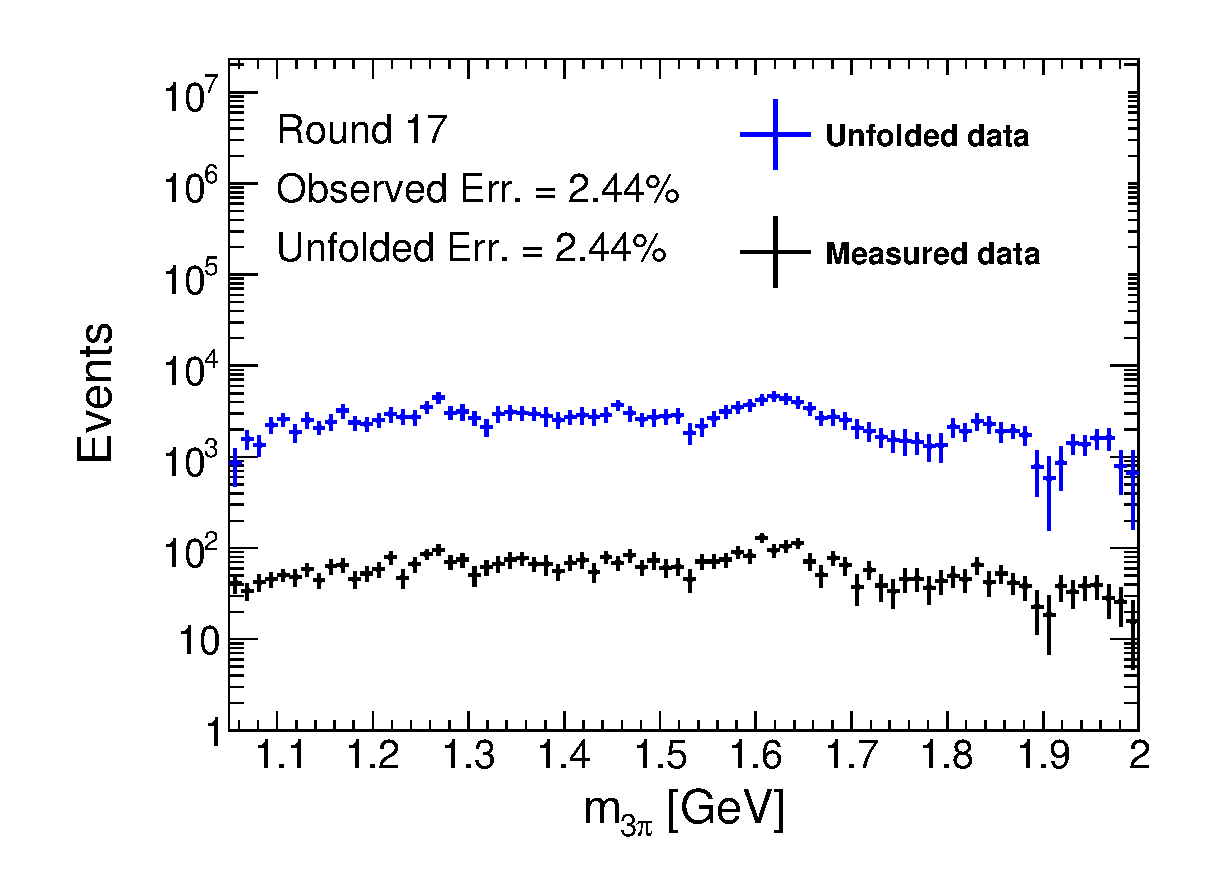
\includegraphics[width=0.32\textwidth]{fig/unfolded_high_round17.eps}
    \label{fig:unfolded_high_r17}
}

\caption{Unfolded $M_{3\pi}$ distributions after applying the corrected response matrix, shown for four data-taking periods. Each row corresponds to a different round: (a)--(c) Round~03/04, (d)--(f) Round~15, (g)--(i) Round~16, and (j)--(l) Round~17. The three columns represent different $3\pi$ invariant mass regions: $\omega(782)$ region (left), $\phi(1020)$ region (center), and higher-mass $\omega^{\prime}/\omega^{\prime\prime}$ region (right). The results are shown only within the nominal mass ranges defined in Tab.~\ref{tab:optimized_parameters}.}
\label{fig:unfolded_data_results_all_rounds}
\end{figure}
